\documentclass[11pt]{llncs}
\usepackage[pdftex]{graphicx}
\usepackage[linesnumbered,ruled,noend]{algorithm2e}
\usepackage[english]{babel}
\usepackage{amsmath}
\let\proof\relax
\let\endproof\relax
\usepackage{amsthm}
\usepackage{mathtools}
\usepackage{amssymb}
\usepackage{lmodern}
\usepackage[T1]{fontenc}
\usepackage{listings}
\usepackage{graphviz}
\usepackage{dot2texi}
\usepackage{tikz}
\usepackage{pgfplots}
\usetikzlibrary{shapes,arrows}
%\usepackage[utf8]{inputenc}
\usepackage{hyperref}
%\usepackage{chngcntr}

\lstset{frame=tb,
  showstringspaces=false,
  columns=flexible,
  basicstyle=\ttfamily,
  keywordstyle=\color{blue},
  commentstyle=\color{dkgreen},
  stringstyle=\color{mauve},
  breaklines=true,
  breakatwhitespace=true,
  tabsize=3,
  escapeinside={(*@}{@*)},
  frame=n
}
\lstdefinestyle{numbers}{numbers=left, stepnumber=1, numberstyle=\tiny, numbersep=10pt}
\let\origthelstnumber\thelstnumber
\makeatletter
\newcommand*\Suppressnumber{%
  \lst@AddToHook{OnNewLine}{%
    \let\thelstnumber\relax%
     \advance\c@lstnumber-\@ne\relax%
    }%
}

\newcommand*\Reactivatenumber{%
  \lst@AddToHook{OnNewLine}{%
   \let\thelstnumber\origthelstnumber%
   \advance\c@lstnumber\@ne\relax}%
}

\def\bitcoin{%
  \leavevmode
  \vtop{\offinterlineskip %\bfseries
    \setbox0=\hbox{B}%
    \setbox2=\hbox to\wd0{\hfil\hskip-.03em
    \vrule height .3ex width .15ex\hskip .08em
    \vrule height .3ex width .15ex\hfil}
    \vbox{\copy2\box0}\box2}}

\makeatletter 
\newcommand\semihuge{\@setfontsize\semihuge{19.22}{23.88}}
\makeatother

%\theoremstyle{definition}
%\newtheorem*{sepproof}{}
%\renewenvironment{sepproof}{{\bfseries Proof}}{}[#1 \bfseries]

\newenvironment{sepproof}[1]{\noindent \textbf{#1}}{\smallskip \ \\}

\renewcommand{\thesubsection}{\arabic{subsection}}

\newenvironment{proofsketch}{\textit{Proof Sketch.}}{\qed \smallskip \ \\}

\pagestyle{plain}

\bibliographystyle{splncs}

% PDF bookmarks
\usepackage{color,hyperref}
\definecolor{darkblue}{rgb}{0.0,0.0,0.3}
\hypersetup{colorlinks,breaklinks,
    linkcolor=darkblue,urlcolor=darkblue,
    anchorcolor=darkblue,citecolor=darkblue}

\begin{document}
\title{Trust Is Risk: \\ A Decentralized Financial Trust Platform}
\author{Anonymized submission}
\institute{}
%\author{Orfeas Stefanos Thyfronitis Litos\inst{1}% \fnmsep \thanks{We thank Kyriakos Axiotis for his insights on flows.}
%        \and Dionysis Zindros\inst{2} \fnmsep \thanks{Research supported by ERC project CODAMODA, project \#259152}}
%\institute{National Technical University of Athens \and National and Kapodistrian University of Athens \\
%           \email{olitos@corelab.ntua.gr}, \email{dionyziz@di.uoa.gr}}
\maketitle
\thispagestyle{plain}
  \begin{abstract}
     Reputation in centralized systems uses stars and review-based trust. Such systems require manual intervention and
     secrecy to avoid manipulation. In autonomous and open source decentralized systems this luxury is not available.
     Previous peer-to-peer reputation systems do not allow for financial arguments pertaining to reputation. We propose a
     concrete Sybil-resilient decentralized reputation system where direct trust is defined as lines-of-credit using
     bitcoin's 1-of-2 multisig. We introduce a new model for bitcoin wallets in which user coins are split among trusted
     associates. Indirect trust is subsequently defined transitively. This enables formal game theoretic arguments pertaining
     to risk analysis. We prove that risk and max flows are equivalent in our model. Our system allows for concrete financial
     decisions on the monetary amount a pseudonymous party can be trusted with. Through algorithmic trust redistribution, the
     risk incurred from making a purchase from a pseudonymous party in this manner remains invariant.
     \keywords{decentralized $\cdot$ trust $\cdot$ web-of-trust $\cdot$ bitcoin $\cdot$ multisig $\cdot$ line-of-credit
               $\cdot$ trust-as-risk $\cdot$ flow $\cdot$ reputation}
  \end{abstract}

  \section{Introduction}
     Modern online marketplaces can be roughly categorized as centralized and decentralized.
     Two major examples of each category are \href{http://www.ebay.com}{ebay} and \href{https://openbazaar.org/}{OpenBazaar}.
     The common denominator of established online marketplaces is that the reputation of each vendor and client is either
     expressed in the form of stars and user-generated reviews that are viewable by the whole network, or not expressed at
     all inside the marketplace and instead is entirely built on word-of-mouth or other out-of-band means.

     Our goal is to create a decentralized marketplace where the trust each user gives to the rest of the users is
     quantifiable, measurable and expressable in monetary terms. The central concept used throughout this paper is
     that trust is equivalent to risk, or the proposition that $Alice$'s \textit{trust} to another user $Bob$ is defined to
     be the \textit{maximum sum of money} that $Alice$ can lose when $Bob$ is free to choose any strategy he wants. To flesh
     out this concept, we will use \textit{lines of credit} as proposed by Washington Sanchez \cite{loc}, not to be confused
     with the synonymous financial product. Joining the network
     will be done by explicitly entrusting a certain amount of money to another user, say $Bob$. If $Bob$ has already
     entrusted an amount of money to a third user, $Charlie$, then we indirectly trust $Charlie$ since if the latter wished
     to play unfairly, he could have already stolen the money entrusted to him by $Bob$. Thus we can engage in economic
     interaction with $Charlie$. The currency used is Bitcoin \cite{bitcoin}. \medskip \ \\
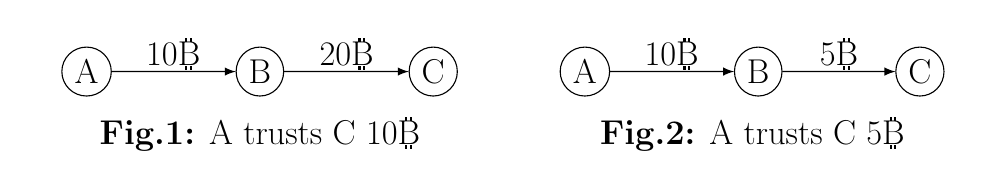
\begin{tikzpicture}[>=latex,line join=bevel,scale=0.60,transform shape]
%%
\begin{scope}
  \pgfsetstrokecolor{black}
  \definecolor{strokecol}{rgb}{1.0,1.0,1.0};
  \pgfsetstrokecolor{strokecol}
  \draw (8.0bp,8.0bp) -- (8.0bp,83.0bp) -- (286.0bp,83.0bp) -- (286.0bp,8.0bp) -- cycle;
  \definecolor{strokecol}{rgb}{0.0,0.0,0.0};
  \pgfsetstrokecolor{strokecol}
  \draw (147.0bp,19.5bp) node {\semihuge \textbf{Fig.1:} A trusts C 10\bitcoin};
\end{scope}
\begin{scope}
  \pgfsetstrokecolor{black}
  \definecolor{strokecol}{rgb}{1.0,1.0,1.0};
  \pgfsetstrokecolor{strokecol}
  \draw (307.0bp,8.0bp) -- (307.0bp,83.0bp) -- (578.0bp,83.0bp) -- (578.0bp,8.0bp) -- cycle;
  \definecolor{strokecol}{rgb}{0.0,0.0,0.0};
  \pgfsetstrokecolor{strokecol}
  \draw (442.5bp,19.5bp) node {\semihuge \textbf{Fig.2:} A trusts C 5\bitcoin};
\end{scope}
  \node (Alice2) at (342.0bp,57.0bp) [draw,ellipse] {\semihuge A};
  \node (Alice1) at (43.0bp,57.0bp) [draw,ellipse] {\semihuge A};
  \node (Charlie2) at (543.0bp,57.0bp) [draw,ellipse] {\semihuge C};
  \node (Charlie1) at (251.0bp,57.0bp) [draw,ellipse] {\semihuge C};
  \node (Bob2) at (446.0bp,57.0bp) [draw,ellipse] {\semihuge B};
  \node (Bob1) at (147.0bp,57.0bp) [draw,ellipse] {\semihuge B};
  \draw [->] (Bob1) -- (Charlie1);
  \draw (199.0bp,67.5bp) node {\semihuge 20\bitcoin};
  \draw [->] (Alice2) -- (Bob2);
  \draw (394.0bp,67.5bp) node {\semihuge 10\bitcoin};
  \draw [->] (Alice1) -- (Bob1);
  \draw (95.0bp,67.5bp) node {\semihuge 10\bitcoin};
  \draw [->] (Bob2) -- (Charlie2);
  \draw (494.5bp,67.5bp) node {\semihuge 5\bitcoin};
%
\end{tikzpicture} \smallskip \ \\
     We thus propose a new kind of wallet where coins are not stored locally, but are placed in 1-of-2 multisigs, a bitcoin
     construction that permits any one of two pre-designated users to spend the coins contained therein
     \cite{masteringbitcoin}. We will use the notation 1/$\{Alice, Bob\}$ to represent a 1-of-2 multisig that can be spent by
     either $Alice$ or $Bob$.

     Our approach changes the user experience in a subtle but drastic way. A user no more has to base her trust towards a
     store on stars, ratings or other dubious and non-quantifiable trust metrics. She can simply consult her wallet to
     decide whether the store is trustworthy and, if so, up to what value. This system works as follows: Initially $Alice$
     migrates her funds from P2PKH addresses in the UTXO \cite{masteringbitcoin} to 1-of-2 multisig addresses shared with
     friends she comfortably trusts. We call this direct trust. Our system is agnostic to the means players use to determine
     who is trustworthy for these direct 1-of-2 deposits.

     Suppose that $Alice$ is viewing the item listings of vendor $Charlie$. Instead of $Charlie$'s stars, $Alice$ will see a
     positive value that is calculated by her wallet and represents the maximum monetary value that $Alice$ can safely use to
     complete a purchase from $Charlie$. We examine exactly how this value is calculated in Trust Flow theorem
     (\ref{trustflow}). This monetary value reported by our system maintains the desired security property that, if $Alice$
     makes this purchase, then she is exposed to no more risk than she was willing to expose herself towards her friends.
     We prove this result in the Risk Invariance theorem (\ref{riskinv}). Obviously it will not be safe for $Alice$ to buy
     anything from $Charlie$ or any other vendor if she has entrusted no value to any other player.

     We see that in TrustIsRisk the money is not invested at the time of the purchase and directly to the vendor, but at an
     earlier point in time and only to parties that are trustworthy for out-of-band reasons. The fact that this system can
     function in a completely decentralized fashion will become clear in the following sections. We prove this result in the
     Sybil Resilience theorem (\ref{sybil}).

     There are several incentives for a user to join this network. First of all, she can have access to a store that is
     otherwise inaccessible. Moreover, two friends can formalize their mutual trust by entrusting the same amount to each
     other. A large company that casually subcontracts other companies to complete various tasks can express its trust
     towards them using this method. A government can choose to entrust its citizens with money and confront them using a
     corresponding legal arsenal if they make irresponsible use of this trust. A bank can provide loans as outgoing and
     manage savings as incoming trust and thus has a unique opportunity of expressing in a formal and absolute way its
     credence by publishing its incoming and outgoing trust. Last but not least, the network can be viewed as a possible
     field for investment and speculation since it constitutes a completely new area for financial activity.

     It is worth noting that the same physical person can maintain multiple pseudonymous identities in the same trust network
     and that multiple independent trust networks for different purposes can coexist. On the other hand, the same
     pseudonymous identity can be used to establish trust in different contexts.
  \section{The Trust Graph}
     We now engage in the formal description of the proposed system, accompanied by helpful examples.
     \begin{definition}[Graph]
        TrustIsRisk is represented by a sequence of directed weighted graphs $\left(\mathcal{G}_j\right)$ where $\mathcal{G}_j
        = \left(\mathcal{V}_j, \mathcal{E}_j\right), j \in \mathbb{N}$.
        Also, since the graphs are weighted, there exists a sequence of weight functions $\left(c_j\right)$ with $c_j :
        \mathcal{E}_j \rightarrow \mathbb{R}^{+}$.
     \end{definition}
     The nodes represent the players, the edges represent the existing direct trusts and the weights represent the amount of
     value attached to the corresponding direct trust. As we will see, the game evolves in turns. The subscript of the graph
     represents the corresponding turn.
     \begin{definition}[Players]
        The set $\mathcal{V}_j = \mathcal{V}\left(\mathcal{G}_j\right)$ is the set of all players in the network, otherwise
        understood as the set of all pseudonymous identities.
     \end{definition}
     Each node has a corresponding non-negative number that represents its capital. A node's capital is the total value that
     the node possesses exclusively and nobody else can spend.
     \begin{definition}[Capital]
        The initial capital of $A$, $Cap_{A, 0}$, is defined as the total value that belongs to $A$ and exists in P2PKH in
        the UTXO at the beginning of the game.
%        The capital of $A$ at the end of turn $j$, $Cap_{A, j}$, is defined as the total value that exists in P2PKH in the
%        UTXO and can be spent by $A$ at the end of turn $j$.
     \end{definition}
     The capital of $A$ is subsequently modified only during her turns, according to her actions. We also note that a
     player's assets are the sum of her capital and her total outgoing trust.

%     \begin{definition}[Assets]
%        Sum of $A$'s capital and outgoing trust.
%        \begin{equation}
%           As_{A, j} = Cap_{A, j} + out_{A, j}
%        \end{equation}
%     \end{definition}
%     We consider the outgoing trust of a player as part of her assets.
     The formal definition of direct trust follows:
     \begin{definition}[Direct Trust]
        Direct trust from $A$ to $B$ at the end of turn $j$, $DTr_{A \rightarrow B, j}$, is defined as the total amount of
        value that exists in 1/$\{A,B\}$ multisigs in the UTXO in the end of turn $j$, where the money is deposited by $A$.
        \begin{equation}
           DTr_{A \rightarrow B, j} =
              \begin{cases}
                 c_j\left(A, B\right), & if \left(A, B\right) \in \mathcal{E}_j \\
                 0, & else
              \end{cases}
        \end{equation}
     \end{definition}
     This definition agrees with the title of this paper and coincides with the intuition and experimental results of
     \cite{kmrs} that the trust $Alice$ shows to $Bob$ in real-world social networks corresponds with the extent
     of danger in which $Alice$ is ready to expose herself to in order to help $Bob$. An example graph with its corresponding
     transactions in the UTXO can be seen below.

     \begin{center}
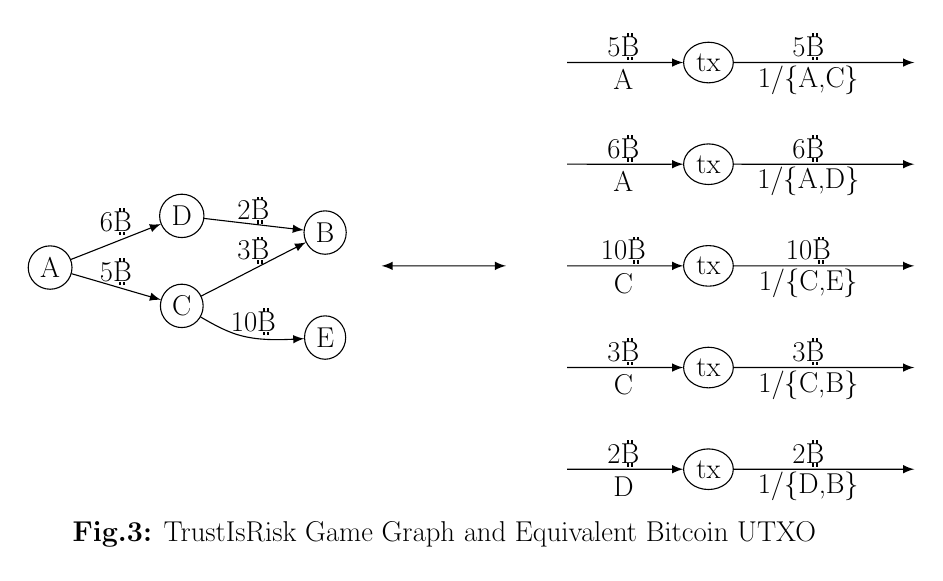
\begin{tikzpicture}[>=latex,line join=bevel,scale=0.6,transform shape]
%%
  \coordinate (Z4) at (344.19bp,100.0bp);
  \coordinate (Z5) at (344.19bp,39.0bp);
  \coordinate (Z1) at (344.19bp,283.0bp);
  \coordinate (Z2) at (344.19bp,222.0bp);
  \coordinate (Z3) at (344.19bp,161.0bp);
  \node (A) at (34.0bp,160.0bp) [draw,ellipse] {\LARGE A};
  \node (C) at (113.0bp,137.0bp) [draw,ellipse] {\LARGE C};
  \node (B) at (199.0bp,181.0bp) [draw,ellipse] {\LARGE B};
  \node (E) at (199.0bp,118.0bp) [draw,ellipse] {\LARGE E};
  \node (D) at (113.0bp,191.0bp) [draw,ellipse] {\LARGE D};
  \node (a1) at (428.99bp,283.0bp) [draw,ellipse] {\LARGE tx};
  \node (a3) at (428.99bp,161.0bp) [draw,ellipse] {\LARGE tx};
  \node (a2) at (428.99bp,222.0bp) [draw,ellipse] {\LARGE tx};
  \node (a5) at (428.99bp,39.0bp) [draw,ellipse] {\LARGE tx};
  \node (a4) at (428.99bp,100.0bp) [draw,ellipse] {\LARGE tx};
  \coordinate (J1) at (232.85bp,161.0bp);
  \coordinate (J2) at (307.54bp,161.0bp);
  \coordinate (Y1) at (552.44bp,283.0bp);
  \coordinate (Y3) at (552.44bp,161.0bp);
  \coordinate (Y2) at (552.44bp,222.0bp);
  \coordinate (Y5) at (552.44bp,39.0bp);
  \coordinate (Y4) at (552.44bp,100.0bp);
  \draw [->] (a4) ..controls (445.3bp,100.0bp) and (461.02bp,100.0bp)  .. (Y4);
  \draw (488.99bp,89.5bp) node {\LARGE 1/\{C,B\}};
  \draw (488.99bp,109.5bp) node {\LARGE 3\bitcoin};
  \draw [->] (Z3) ..controls (377.14bp,161.0bp) and (392.28bp,161.0bp)  .. (a3);
  \draw (377.99bp,150.5bp) node {\LARGE C};
  \draw (377.99bp,170.5bp) node {\LARGE 10\bitcoin};
  \draw [->] (a3) ..controls (445.3bp,161.0bp) and (461.02bp,161.0bp)  .. (Y3);
  \draw (488.99bp,150.5bp) node {\LARGE 1/\{C,E\}};
  \draw (488.99bp,170.5bp) node {\LARGE 10\bitcoin};
  \draw [<->] (J1) ..controls (265.65bp,161.0bp) and (274.33bp,161.0bp)  .. (J2);
  \draw [->] (a2) ..controls (445.3bp,222.0bp) and (541.02bp,222.0bp)  .. (Y2);
  \draw (488.99bp,211.5bp) node {\LARGE 1/\{A,D\}};
  \draw (488.99bp,231.5bp) node {\LARGE 6\bitcoin};
  \draw [->] (C) ..controls (134.77bp,124.17bp) and (141.98bp,120.776bp)  .. (149.0bp,119.0bp) .. controls (157.28bp,116.905bp) and (166.61bp,116.3bp)  .. (E);
  \draw (156.0bp,127.5bp) node {\LARGE 10\bitcoin};
  \draw [->] (a5) ..controls (445.3bp,39.0bp) and (541.02bp,39.0bp)  .. (Y5);
  \draw (488.99bp,28.5bp) node {\LARGE 1/\{D,B\}};
  \draw (488.99bp,48.5bp) node {\LARGE 2\bitcoin};
  \draw [->] (C) ..controls (142.79bp,152.08bp) and (162.28bp,162.29bp)  .. (B);
  \draw (156.0bp,170.5bp) node {\LARGE 3\bitcoin};
  \draw [->] (Z5) ..controls (377.14bp,39.0bp) and (392.28bp,39.0bp)  .. (a5);
  \draw (377.99bp,28.5bp) node {\LARGE D};
  \draw (377.99bp,48.5bp) node {\LARGE 2\bitcoin};
  \draw [->] (Z2) ..controls (377.14bp,222.0bp) and (392.28bp,222.0bp)  .. (a2);
  \draw (377.99bp,211.5bp) node {\LARGE A};
  \draw (377.99bp,231.5bp) node {\LARGE 6\bitcoin};
  \draw [->] (A) ..controls (62.311bp,171.0bp) and (77.709bp,177.19bp)  .. (D);
  \draw (73.5bp,187.5bp) node {\LARGE 6\bitcoin};
  \draw [->] (a1) ..controls (445.3bp,283.0bp) and (541.02bp,283.0bp)  .. (Y1);
  \draw (488.99bp,272.5bp) node {\LARGE 1/\{A,C\}};
  \draw (488.99bp,292.5bp) node {\LARGE 5\bitcoin};
  \draw [->] (Z4) ..controls (377.14bp,100.0bp) and (392.28bp,100.0bp)  .. (a4);
  \draw (377.99bp,89.5bp) node {\LARGE C};
  \draw (377.99bp,109.5bp) node {\LARGE 3\bitcoin};
  \draw [->] (A) ..controls (62.483bp,151.79bp) and (77.403bp,147.33bp)  .. (C);
  \draw (73.5bp,157.5bp) node {\LARGE 5\bitcoin};
  \draw [->] (Z1) ..controls (377.14bp,283.0bp) and (392.28bp,283.0bp)  .. (a1);
  \draw (377.99bp,272.5bp) node {\LARGE A};
  \draw (377.99bp,292.5bp) node {\LARGE 5\bitcoin};
  \draw [->] (D) ..controls (143.64bp,187.47bp) and (161.02bp,185.4bp)  .. (B);
  \draw (156.0bp,194.5bp) node {\LARGE 2\bitcoin};
  \draw (270.5bp,0.0bp) node {\LARGE \textbf{Fig.3:} TrustIsRisk Game Graph and Equivalent Bitcoin UTXO};
%
\end{tikzpicture}
     \end{center}

     Any algorithm that has access to the graph $\mathcal{G}_j$ has implicitly access to all direct trusts of this graph.
     We use the notation $N^{+}(A)$ to refer to the nodes directly trusted by $A$ and $N^{-}(A)$ for the nodes that directly
     trust $A$. We also use the notation $in_{A, j}, out_{A, j}$ to refer to the total incoming and outgoing direct trust
     respectively. For a reference of common definitions, see the Appendix.
   \section{Evolution of Trust}
     \begin{definition}[Turns]
        The game is turn-based. In each turn $j$ a player $A \in \mathcal{V}, A =
        Player\left(j\right)$, chooses one or more actions from the following two kinds:

        \noindent \textit{\textbf{Steal($y_B$,$\:B$)}}: Steal value $y_B$ from $B \in N^{-}\left(A\right)_{j-1}$, where
        $0 \leq y_B \leq DTr_{B \rightarrow A, j-1}$. Then:
        \begin{equation*}
           DTr_{B \rightarrow A, j} = DTr_{B \rightarrow A, j-1} - y_B
        \end{equation*}
        \noindent \textit{\textbf{Add($y_B$,$\:B$)}}:
        Add value $y_B$ to $B \in \mathcal{V}$, where $-DTr_{A \rightarrow B, j-1} \leq y_B$. Then:
        \begin{equation*}
           DTr_{A \rightarrow B, j} = DTr_{A \rightarrow B, j-1} + y_B
        \end{equation*}
        When $y_B < 0$, we say that $A$ reduces her trust to $B$ by $-y_B$. When $y_B > 0$, we say that $A$ increases her
        trust to $B$ by $y_B$. If $DTr_{A \rightarrow B, j-1} = 0$, then we say that $A$ starts directly trusting $B$.
        $A$ passes her turn if she chooses no action. Also, let $Y_{st}, Y_{add}$ be the
        total value to be stolen and added respectively by $A$ in her turn, $j$. For a turn to be feasible, it must hold
        \begin{equation}
           Y_{add} - Y_{st} \leq Cap_{A, j-1} \enspace.
        \end{equation}
        The capital is updated in every turn: $Cap_{A, j} = Cap_{A, j-1} + Y_{st} - Y_{add}$.

        A player cannot choose two actions of the same kind against the same player in one turn.
        The set of actions of a player in turn $j$ is denoted by $Turn_j$. The graph that emerges by applying
        the actions on $\mathcal{G}_{j-1}$ is $\mathcal{G}_j$.
     \end{definition}
     We use $prev\left(j\right)$ and $next\left(j\right)$ to denote the previous and next turn respectively played by
     $Player(j)$. A formal definition is in the Appendix.
     \begin{definition}[Damage]
        Let $j$ be a turn such that $Player\left(j\right) = A$.
        \begin{equation}
           Damage_{A, j} = out_{A, prev\left(j\right)} - out_{A, j-1}
        \end{equation}
        We say that $A$ has been stolen value $Damage_{A, j}$ between $prev\left(j\right)$ and $j$. We omit turn subscripts
        if they are implied from the context.
     \end{definition}
     \begin{definition}[History]
        We define History, $\mathcal{H} = \left(\mathcal{H}_j\right)$, as the sequence of all tuples containing the sets
        of actions and the corresponding player.
        \begin{equation}
           \mathcal{H}_j = \left(Player\left(j\right), Turn_j\right)
        \end{equation}
     \end{definition}
     Knowledge of the initial graph $\mathcal{G}_0$ and the history amount to full comprehension of the evolution of the
     game. Building on the example of Figure 3, we can see the resulting graph when $D$ plays
     \begin{equation}
     \label{turnexample}
        Turn_1 = \{Steal\left(1, A\right), Add\left(4, C\right)\} \enspace.
     \end{equation}
\begin{center}
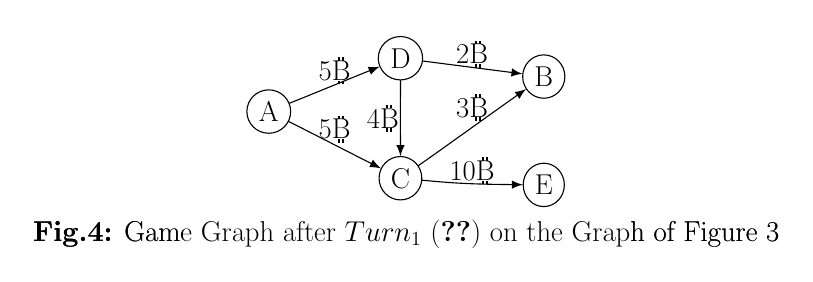
\begin{tikzpicture}[>=latex,line join=bevel,scale=0.6,transform shape]
%%
\begin{scope}
  \definecolor{strokecol}{rgb}{0.0,0.0,0.0};
  \pgfsetstrokecolor{strokecol}
  \draw (133.5bp,11.5bp) node {\LARGE \textbf{Fig.4:} Game Graph after $Turn_1$ (\ref{turnexample}) on the Graph of Figure 3};
\end{scope}
\begin{scope}
  \pgfsetstrokecolor{black}
  \definecolor{strokecol}{rgb}{1.0,1.0,1.0};
  \pgfsetstrokecolor{strokecol}
  \definecolor{fillcol}{rgb}{1.0,1.0,1.0};
  \pgfsetfillcolor{fillcol}
  \filldraw (0.0bp,0.0bp) -- (0.0bp,135.0bp) -- (267.0bp,135.0bp) -- (267.0bp,0.0bp) -- cycle;
  \definecolor{strokecol}{rgb}{0.0,0.0,0.0};
  \pgfsetstrokecolor{strokecol}
  \draw (133.5bp,11.5bp) node {\LARGE \textbf{Fig.4:} Game Graph after $Turn_1$ (\ref{turnexample}) on the Graph of Figure 3};
\end{scope}
  \node (A) at (51.0bp,85.0bp) [draw,ellipse] {\LARGE A};
  \node (C) at (130.0bp,45.0bp) [draw,ellipse] {\LARGE C};
  \node (B) at (216.0bp,106.0bp) [draw,ellipse] {\LARGE B};
  \node (E) at (216.0bp,41.0bp) [draw,ellipse] {\LARGE E};
  \node (D) at (130.0bp,117.0bp) [draw,ellipse] {\LARGE D};
  \draw [->] (C) ..controls (153.77bp,42.809bp) and (160.15bp,42.31bp)  .. (166.0bp,42.0bp) .. controls (174.23bp,41.564bp) and (183.25bp,41.314bp)  .. (E);
  \draw (173.0bp,49.5bp) node {\LARGE 10\bitcoin};
  \draw [->] (C) ..controls (159.21bp,65.487bp) and (180.58bp,81.004bp)  .. (B);
  \draw (173.0bp,87.5bp) node {\LARGE 3\bitcoin};
  \draw [->] (A) ..controls (79.311bp,96.35bp) and (94.709bp,102.75bp)  .. (D);
  \draw (90.5bp,109.5bp) node {\LARGE 5\bitcoin};
  \draw [->] (D) ..controls (130.0bp,89.666bp) and (130.0bp,78.836bp)  .. (C);
  \draw (119.5bp,81.0bp) node {\LARGE 4\bitcoin};
  \draw [->] (A) ..controls (78.919bp,71.016bp) and (95.226bp,62.545bp)  .. (C);
  \draw (90.5bp,74.5bp) node {\LARGE 5\bitcoin};
  \draw [->] (D) ..controls (160.64bp,113.12bp) and (178.02bp,110.84bp)  .. (B);
  \draw (173.0bp,119.5bp) node {\LARGE 2\bitcoin};
%
\end{tikzpicture}
\end{center}
     TrustIsRisk is controlled by an algorithm that chooses a player, receives the turn that
     this player wishes to play and, if this turn is valid, executes it. These steps are repeated indefinitely. We assume
     players are chosen in a way that, after her turn, a player will eventually play again later.
     \Suppressnumber
     \begin{lstlisting}[label=trustisriskgame, style=numbers]
TrustIsRisk Game (*@\Reactivatenumber@*)
j = 0
while (True)
  j += 1;  (*@$v \overset{\$}{\gets} \mathcal{V}_j$@*)
  Turn = (*@$v$@*)Strategy((*@$\mathcal{G}_0$@*), (*@$v$@*), (*@$\left(\mathcal{H}\right)_{1 \dots j-1}$@*))
  ((*@$\mathcal{G}_j$@*), (*@$Cap_{v, j}$@*), (*@$\mathcal{H}_j$@*)) = executeTurn((*@$\mathcal{G}_{j-1}$@*), (*@$v$@*), (*@$Cap_{v, j-1}$@*), Turn)
    \end{lstlisting}
%    This algorithm calls the necessary functions to prepare the new graph.
%    \Suppressnumber
%    \begin{lstlisting}[label=executeturn, style=numbers]
%Execute Turn
%Input : old graph (*@$\mathcal{G}_{j-1}$@*), player (*@$A \in \mathcal{V}_{j-1}$@*), old capital (*@$Cap_{A, j-1}$@*), TentativeTurn
%Output : new graph (*@$\mathcal{G}_j$@*), new capital (*@$Cap_{A, j}$@*), new history (*@$\mathcal{H}_j$ \Reactivatenumber@*)
%executeTurn((*@$\mathcal{G}_{j-1}$@*), (*@$A$@*), (*@$Cap_{A, j-1}$@*), TentativeTurn) :
%  ((*@$Turn_j$@*), NewCap) = validateTurn((*@$\mathcal{G}_{j-1}$@*), (*@$A$@*), (*@$Cap_{A, j-1}$@*), TentativeTurn)
%  return(commitTurn((*@$\mathcal{G}_{j-1}$@*), (*@$A$@*), (*@$Turn_j$@*), NewCap))
%    \end{lstlisting}
     \texttt{executeTurn()} checks the validity of \texttt{Turn} and substitutes it with an empty turn if invalid.
     Subsequently, it creates the new graph $\mathcal{G}_j$ and updates the history accordingly. For the routine code,
     see the Appendix.
  \section{Trust Transitivity}
     In this section we define some strategies. The corresponding algorithms can be seen in the Appendix. Then we define the
     Transitive Game that represents the worst-case scenario for an honest player when another player decides to depart from
     the network with her money and all the money entrusted to her.
     \begin{definition}[Idle Strategy]
        A player $A$ is said to follow the idle strategy if she passes in her turn. 
     \end{definition}

     \Suppressnumber
     \begin{lstlisting}[label=idlestrategy, style=numbers]
Idle Strategy
Input : initial graph (*@$\mathcal{G}_0$@*), player (*@$A$@*), history (*@$\left(\mathcal{H}\right)_{1 \dots j-1}$@*)
Output : (*@$Turn_j$ \Reactivatenumber@*)
idleStrategy((*@$\mathcal{G}_0$@*), (*@$A$@*), (*@$\mathcal{H}$@*)) :
  return((*@$\emptyset$@*))
     \end{lstlisting}
     The inputs and outputs are identical to those of \texttt{idleStrategy()} for the rest of the strategies, thus we avoid
     repeating them.
     \begin{definition}[Evil Strategy]
        A player $A$ is said to follow the evil strategy if she steals all incoming direct trust and nullifies her outgoing
        direct trust in her turn.
     \end{definition}

     \begin{lstlisting}[label=evilstrategy, style=numbers]
evilStrategy((*@$\mathcal{G}_0$@*), (*@$A$@*), (*@$\mathcal{H}$@*)) :
  Steals = (*@$\bigcup\limits_{v \in N^{-}\left(A\right)_{j-1}}\{Steal(DTr_{v \rightarrow A, j-1}, v)\}$@*)
  Adds = (*@$\bigcup\limits_{v \in N^{+}\left(A\right)_{j-1}}\{Add(-DTr_{A \rightarrow v, j-1}, v)\}$@*)
  (*@$Turn_j$@*) = Steals(*@$\: \cup \:$@*)Adds
  return((*@$Turn_j$@*))
     \end{lstlisting}

     \begin{definition}[Conservative Strategy]
        Player $A$ is said to follow the conservative strategy if she replenishes the value she lost since the previous turn,
        $Damage_A$, by stealing from others that trust her as much as she can up to $Damage_A$ and she takes no other action.
     \end{definition}

     \begin{lstlisting}[label=conservativestrategy, style=numbers]
consStrategy((*@$\mathcal{G}_0$@*), (*@$A$@*), (*@$\mathcal{H}$@*)) :
  Damage = (*@$out_{A, prev\left(j\right)}$@*) - (*@$out_{A, j-1}$@*)
  if (Damage > 0)
    if (Damage >= (*@$in_{A, j-1}$@*))
      (*@$Turn_j$@*) = (*@$\bigcup\limits_{v \in N^{-}\left(A\right)_{j-1}}\{Steal\left(DTr_{v \rightarrow A, j-1}, v\right)\}$@*)
    else
      (*@$y$@*) = SelectSteal((*@$G_j$@*), (*@$A$@*), Damage)    #(*@$y$@*) = (*@$\{y_v : v \in N^{-}\left(A\right)_{j-1}\}$@*)
      (*@$Turn_j$@*) = (*@$\bigcup\limits_{v \in N^{-}\left(A\right)_{j-1}}\{Steal\left(y_v, v\right)\}$@*)
  else (*@$Turn_j$@*) = (*@$\emptyset$@*)
  return((*@$Turn_j$@*))
     \end{lstlisting}
     \texttt{SelectSteal()} returns $y_v$ with $v \in N^{-}\left(A\right)_{j-1}$ such that
     \begin{equation}
     \label{stealrestriction}
        \sum\limits_{v \in N^{-}\left(A\right)_{j-1}}y_v = Damage_{A, j} \wedge \forall v \in N^{-}\left(A\right)_{j-1},
        y_v \leq DTr_{v \rightarrow A, j-1} \enspace.
     \end{equation}
     Player $A$ can arbitrarily define how \texttt{SelectSteal()} distributes the $Steal\left(\right)$ actions
     each time she calls the function, as long as (\ref{stealrestriction}) is respected. 

     As we can see, the definition covers a multitude of options for the conservative player, since in case $0 < Damage_{A,j}
     < in_{A,j-1}$ she can choose to distribute the $Steal\left(\right)$ actions in any way she chooses.

     The rationale behind this strategy arises from a real-world common situation. Suppose there are a client, an
     intermediary and a producer. The client entrusts some value to the intermediary so that the latter can buy the desired
     product from the producer and deliver it to the client. The intermediary in turn entrusts an equal value to the
     producer, who needs the value upfront to be able to complete the production process. However the producer eventually
     does not give the product neither reimburses the value, due to bankruptcy or decision to exit the market with an unfair
     benefit. The intermediary can choose either to reimburse the client and suffer the loss, or refuse to return the money
     and lose the client's trust. The latter choice for the intermediary is exactly the conservative strategy. It is used
     throughout this work as a strategy for all the intermediary players because it models effectively the worst-case
     scenario that a client can face after an evil player decides to steal everything she can and the rest of the players do
     not engage in evil activity.

     We continue with a very useful possible evolution of the game, the Transitive Game. In turn 0, there is already a network
     in place. All players apart from $A$ and $E$ follow the conservative strategy. Furthermore, the set of players is not
     modified throughout the Transitive Game, thus we can refer to $\mathcal{V}_j$ for any turn $j$ as $\mathcal{V}$.
     Moreover, each conservative player can be in one of three states: Happy, Angry or Sad. Happy players have 0 loss, Angry
     players have positive loss and positive incoming trust, thus are able to replenish their loss at least in part and
     Sad players have positive loss, but 0 incoming trust, thus they cannot replenish the loss. These conventions will hold
     whenever we use the Transitive Game.
% For the algorithm, see the Appendix.
     \Suppressnumber
     \begin{lstlisting}[label=transitivegame, style=numbers]
Transitive Game
Input : graph (*@$\mathcal{G}_0$@*), (*@$A \in \mathcal{V}$@*) idle player, (*@$E \in \mathcal{V}$@*) evil player (*@\Reactivatenumber@*)
Angry = Sad = (*@$\emptyset$@*) (*@\label{trstealsadinit}@*);  Happy = (*@$\mathcal{V} \setminus \{A, E\}$@*)
for ((*@$v \in \mathcal{V} \setminus \{E\}$@*))  (*@$Loss_v$@*) = 0 (*@\label{trsteallossinit}@*)
j = 0
while (True)
  j += 1;  (*@$v \overset{\$}{\gets} \mathcal{V} \setminus \{A\}$@*)
  (*@$Turn_j$@*) = (*@$v$@*)Strategy((*@$\mathcal{G}_0$@*), (*@$v$@*), (*@$\left(\mathcal{H}\right)_{1 \dots j-1}$@*))
  executeTurn((*@$\mathcal{G}_{j-1}$@*), (*@$Cap_{v, j-1}$@*), (*@$Turn_j$@*))
  for (action (*@$\in Turn_j$@*))
    action match do
      case (*@$Steal($@*)y(*@$,w)$@*) do
        exchange = y
        (*@$Loss_w$@*) += exchange (*@\label{trsteallossincrease}@*)
        if ((*@$v$@*) != (*@$E$@*)) (*@$Loss_v$@*) -= exchange (*@\label{trsteallossdecrease}@*)
        if ((*@$w$@*) != (*@$A$@*))
          Happy = Happy(*@$\:\setminus\: \{w\}$@*)
          if ((*@$in_{w, j}$@*) == 0) Sad = Sad(*@$\:\cup\: \{w\}$@*)
          else Angry = Angry(*@$\:\cup\: \{w\}$@*)
  if ((*@$v$@*) != (*@$E$@*))
    Angry = Angry(*@$\:\setminus\: \{v\}$@*)
    if ((*@$Loss_v$@*) > 0) (*@\label{trstealifentersad}@*)  Sad = Sad(*@$\:\cup\: \{v\}$@*)        #(*@$in_{v, j}$@*) should be zero (*@\label{trstealtrueentersad}@*)
    if ((*@$Loss_v$@*) == 0)  Happy = Happy(*@$\:\cup\: \{v\}$@*)
     \end{lstlisting}

     An example execution follows:

\begin{center}
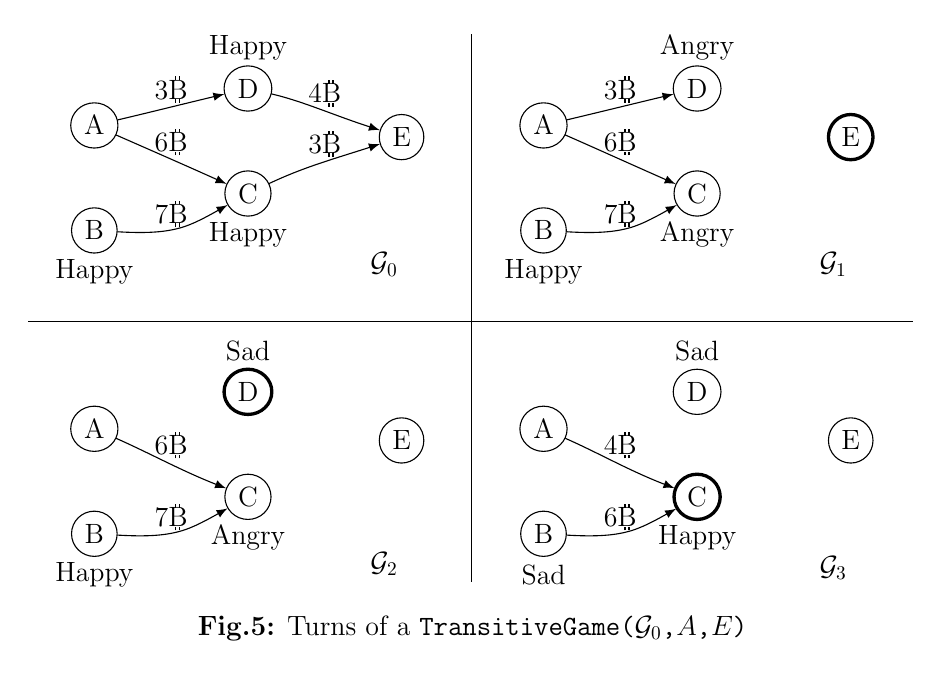
\begin{tikzpicture}[>=latex,line join=bevel,scale=0.7,transform shape]
%%
\begin{scope}
  \definecolor{strokecol}{rgb}{0.0,0.0,0.0};
  \pgfsetstrokecolor{strokecol}
  \draw (228.5bp,11.5bp) node {\Large \textbf{Fig.5:} Turns of a \texttt{TransitiveGame(}$\mathcal{G}_0$\texttt{,}$A$\texttt{,}$E$\texttt{)}};
\end{scope}
\begin{scope}
  \pgfsetstrokecolor{black}
  \definecolor{strokecol}{rgb}{1.0,1.0,1.0};
  \pgfsetstrokecolor{strokecol}
  \definecolor{fillcol}{rgb}{1.0,1.0,1.0};
  \pgfsetfillcolor{fillcol}
  \filldraw (0.0bp,0.0bp) -- (0.0bp,320.0bp) -- (457.0bp,320.0bp) -- (457.0bp,0.0bp) -- cycle;
  \definecolor{strokecol}{rgb}{0.0,0.0,0.0};
  \pgfsetstrokecolor{strokecol}
  \draw (228.5bp,11.5bp) node {\Large \textbf{Fig.5:} Turns of a \texttt{TransitiveGame(}$\mathcal{G}_0$\texttt{,}$A$\texttt{,}$E$\texttt{)}};
\end{scope}
\begin{scope}
  \pgfsetstrokecolor{black}
  \definecolor{strokecol}{rgb}{1.0,1.0,1.0};
  \pgfsetstrokecolor{strokecol}
  \definecolor{fillcol}{rgb}{1.0,1.0,1.0};
  \pgfsetfillcolor{fillcol}
  \filldraw (0.0bp,0.0bp) -- (0.0bp,320.0bp) -- (457.0bp,320.0bp) -- (457.0bp,0.0bp) -- cycle;
  \definecolor{strokecol}{rgb}{0.0,0.0,0.0};
  \pgfsetstrokecolor{strokecol}
  \draw (228.5bp,11.5bp) node {\Large \textbf{Fig.5:} Turns of a \texttt{TransitiveGame(}$\mathcal{G}_0$\texttt{,}$A$\texttt{,}$E$\texttt{)}};
\end{scope}
\begin{scope}
  \pgfsetstrokecolor{black}
  \definecolor{strokecol}{rgb}{1.0,1.0,1.0};
  \pgfsetstrokecolor{strokecol}
  \draw (239.0bp,31.0bp) -- (239.0bp,179.0bp) -- (449.0bp,179.0bp) -- (449.0bp,31.0bp) -- cycle;
  \definecolor{strokecol}{rgb}{0.0,0.0,0.0};
  \pgfsetstrokecolor{strokecol}
  \draw (414.0bp,42.5bp) node {\Large $\mathcal{G}_3$};
\end{scope}
\begin{scope}
  \pgfsetstrokecolor{black}
  \definecolor{strokecol}{rgb}{1.0,1.0,1.0};
  \pgfsetstrokecolor{strokecol}
  \draw (8.0bp,33.0bp) -- (8.0bp,181.0bp) -- (218.0bp,181.0bp) -- (218.0bp,33.0bp) -- cycle;
  \definecolor{strokecol}{rgb}{0.0,0.0,0.0};
  \pgfsetstrokecolor{strokecol}
  \draw (183.0bp,44.5bp) node {\Large $\mathcal{G}_2$};
\end{scope}
\begin{scope}
  \pgfsetstrokecolor{black}
  \definecolor{strokecol}{rgb}{1.0,1.0,1.0};
  \pgfsetstrokecolor{strokecol}
  \draw (239.0bp,187.0bp) -- (239.0bp,320.0bp) -- (449.0bp,320.0bp) -- (449.0bp,187.0bp) -- cycle;
  \definecolor{strokecol}{rgb}{0.0,0.0,0.0};
  \pgfsetstrokecolor{strokecol}
  \draw (414.0bp,198.5bp) node {\Large $\mathcal{G}_1$};
\end{scope}
\begin{scope}
  \pgfsetstrokecolor{black}
  \definecolor{strokecol}{rgb}{1.0,1.0,1.0};
  \pgfsetstrokecolor{strokecol}
  \draw (8.0bp,202.0bp) -- (8.0bp,320.0bp) -- (218.0bp,320.0bp) -- (218.0bp,202.0bp) -- cycle;
  \definecolor{strokecol}{rgb}{0.0,0.0,0.0};
  \pgfsetstrokecolor{strokecol}
  \draw (183.0bp,198.5bp) node {\Large $\mathcal{G}_0$};
\end{scope}
  \node (E3) at (192.0bp,264.0bp) [draw,ellipse] {\Large E};
  \node (E2) at (423.0bp,264.0bp) [draw,ellipse,very thick] {\Large E};
  \node (D2) at (344.0bp,289.0bp) [draw,ellipse] {\Large D};
  \node (D2mood) at (344.0bp,310.0bp) {\Large Angry};
  \node (D3) at (113.0bp,289.0bp) [draw,ellipse] {\Large D};
  \node (D3mood) at (113.0bp,310.0bp) {\Large Happy};
  \node (A1) at (34.0bp,114.0bp) [draw,ellipse] {\Large A};
  \node (A0) at (265.0bp,114.0bp) [draw,ellipse] {\Large A};
  \node (A3) at (34.0bp,270.0bp) [draw,ellipse] {\Large A};
  \node (A2) at (265.0bp,270.0bp) [draw,ellipse] {\Large A};
  \node (B0) at (265.0bp,60.0bp) [draw,ellipse] {\Large B};
  \node (B0mood) at (265.0bp,39.0bp) {\Large Sad};
  \node (B1) at (34.0bp,60.0bp) [draw,ellipse] {\Large B};
  \node (B1mood) at (34.0bp,39.0bp) {\Large Happy};
  \node (B2) at (265.0bp,216.0bp) [draw,ellipse] {\Large B};
  \node (B2mood) at (265.0bp,195.0bp) {\Large Happy};
  \node (B3) at (34.0bp,216.0bp) [draw,ellipse] {\Large B};
  \node (B3mood) at (34.0bp,195.0bp) {\Large Happy};
  \node (C3) at (113.0bp,235.0bp) [draw,ellipse] {\Large C};
  \node (C3mood) at (113.0bp,214.0bp) {\Large Happy};
  \node (C2) at (344.0bp,235.0bp) [draw,ellipse] {\Large C};
  \node (C2mood) at (344.0bp,214.0bp) {\Large Angry};
  \node (C1) at (113.0bp,79.0bp) [draw,ellipse] {\Large C};
  \node (C1mood) at (113.0bp,58.0bp) {\Large Angry};
  \node (C0) at (344.0bp,79.0bp) [draw,ellipse,very thick] {\Large C};
  \node (C0mood) at (344.0bp,58.0bp) {\Large Happy};
  \node (E1) at (192.0bp,108.0bp) [draw,ellipse] {\Large E};
  \node (E0) at (423.0bp,108.0bp) [draw,ellipse] {\Large E};
  \node (D0) at (344.0bp,133.0bp) [draw,ellipse] {\Large D};
  \node (D0mood) at (344.0bp,154.0bp) {\Large Sad};
  \node (D1) at (113.0bp,133.0bp) [draw,ellipse,very thick] {\Large D};
  \node (D1mood) at (113.0bp,154.0bp) {\Large Sad};
  \draw [->] (B1) ..controls (59.732bp,58.525bp) and (68.942bp,58.948bp)  .. (77.0bp,61.0bp) .. controls (82.045bp,62.285bp) and (87.187bp,64.399bp)  .. (C1);
  \draw (73.5bp,68.5bp) node {\Large 7\bitcoin};
  \draw [->] (A3) ..controls (62.101bp,257.65bp) and (78.735bp,250.41bp)  .. (C3);
  \draw (73.5bp,261.5bp) node {\Large 6\bitcoin};
  \draw [->] (A1) ..controls (62.101bp,101.65bp) and (78.735bp,92.41bp)  .. (C1);
  \draw (73.5bp,105.5bp) node {\Large 6\bitcoin};
  \draw [->] (A2) ..controls (293.71bp,276.84bp) and (308.24bp,280.42bp)  .. (D2);
  \draw (304.5bp,288.5bp) node {\Large 3\bitcoin};
  \draw [->] (A0) ..controls (293.17bp,101.65bp) and (309.1bp,92.41bp)  .. (C0);
  \draw (304.5bp,105.5bp) node {\Large 4\bitcoin};
  \draw [->] (B3) ..controls (59.732bp,214.52bp) and (68.942bp,214.95bp)  .. (77.0bp,217.0bp) .. controls (82.045bp,218.28bp) and (87.187bp,220.4bp)  .. (C3);
  \draw (73.5bp,224.5bp) node {\Large 7\bitcoin};
  \draw [->] (B2) ..controls (290.73bp,214.52bp) and (299.94bp,214.95bp)  .. (308.0bp,217.0bp) .. controls (313.04bp,218.28bp) and (318.19bp,220.4bp)  .. (C2);
  \draw (304.5bp,224.5bp) node {\Large 7\bitcoin};
  \draw [->] (A2) ..controls (293.17bp,257.65bp) and (309.1bp,250.41bp)  .. (C2);
  \draw (304.5bp,261.5bp) node {\Large 6\bitcoin};
  \draw [->] (C3) ..controls (141.95bp,248.63bp) and (156.16bp,252.48bp)  .. (E3);
  \draw (152.5bp,260.5bp) node {\Large 3\bitcoin};
  \draw [->] (D3) ..controls (141.1bp,282.51bp) and (157.73bp,275.01bp)  .. (E3);
  \draw (152.5bp,286.5bp) node {\Large 4\bitcoin};
  \draw [->] (A3) ..controls (62.955bp,276.84bp) and (77.158bp,280.42bp)  .. (D3);
  \draw (73.5bp,288.5bp) node {\Large 3\bitcoin};
  \draw [->] (B0) ..controls (290.73bp,58.525bp) and (299.94bp,58.948bp)  .. (308.0bp,61.0bp) .. controls (313.04bp,62.285bp) and (318.19bp,64.399bp)  .. (C0);
  \draw (304.5bp,68.5bp) node {\Large 6\bitcoin};
  \draw (228.0bp,317.0bp) -- (228.0bp,35.0bp);
  \draw (0.0bp,169.0bp) -- (455.0bp,169.0bp);
%
\end{tikzpicture}
\end{center}

     Let $j_0$ be the first turn on which $E$ is chosen to play. Until then, all players will pass their turn since nothing
     has been stolen yet (see the Appendix (theorem \ref{conservativeworld}) for a formal proof of this simple fact).
     Moreover, let $v = Player(j)$ and $j' = prev\left(j\right)$.
%     Given that
%     \begin{equation}
%        Damage_{v,j} = out_{v, j'} - out_{v, j-1} \enspace,
%     \end{equation}
     The Transitive Game generates turns:
     \begin{equation}
        Turn_j = \bigcup\limits_{w \in N^{-}\left(v\right)_{j-1}}\{Steal\left(y_w,w\right)\} \enspace,% Damage_{v, j} > 0 \enspace,
     \end{equation}
     where
     \begin{equation*}
        \sum\limits_{w \in N^{-}\left(v\right)_{j-1}}y_w = \min\left(in_{v, j-1}, Damage_{v, j}\right) \enspace.
     \end{equation*}
 
     We see that if $Damage_{v, j} = 0$, then $Turn_j = \emptyset$.

     From the definition of $Damage_{v,j}$ and knowing that no strategy in this case can increase any direct trust, we see
     that $Damage_{v,j} \geq 0$. Also, it is $Loss_{v,j} \geq 0$ because if $Loss_{v,j} < 0$, then $v$ has
     stolen more value than she has been stolen, thus she would not be following the conservative strategy.
%    In the figure above, $D$ is angry after turn 1 and sad after turn 2 and on. $C$ is angry after turns 1 and 2 and happy
%    after turn 3. $B$ is happy until the end of turn 2 and sad after turn 3. The game converges in turn 4.
  \section{Trust Flow}
    We can now define the indirect trust, or simply trust, from $A$ to $B$.
    \begin{definition}[Indirect Trust]
       The indirect trust from $A$ to $B$ after turn $j$ is defined as the maximum possible value that can be stolen from
       $A$ after turn $j$ in the setting of \texttt{TransitiveGame(}$\mathcal{G}_j$\texttt{,}$A$\texttt{,}$B$\texttt{)}.
    \end{definition}
    \noindent It is $Tr_{A \rightarrow B} \geq DTr_{A \rightarrow B}$. The next theorem shows that
    $Tr_{A \rightarrow B}$ is finite.
    \begin{theorem}[Trust Convergence Theorem] \ \\
       \label{convergence}
       Consider a Transitive Game. There exists a turn such that all subsequent turns are empty.
%       \begin{equation*}
%          \forall j \geq j', Turn_j = \emptyset \enspace.
%       \end{equation*}
    \end{theorem}
    \begin{proofsketch}
       If the game didn't converge, the $Steal\left(\right)$ actions would continue forever without reduction of the amount
       stolen over time, thus they would reach infinity. However this is impossible, since there exists only finite total
       trust.
    \end{proofsketch}
    Full proofs of all theorems and lemmas can be found in the Appendix.

    In the setting of \texttt{TransitiveGame(}$\mathcal{G}$\texttt{,}$A$\texttt{,}$E$\texttt{)}, we make use of the notation
    $Loss_A = Loss_{A, j}$, where $j$ is a turn that the game has converged. It is important to note that $Loss_A$ is
    not the same for repeated executions of this kind of game, since the order in which players are chosen may differ between
    executions and the conservative players are free to choose which incoming trusts they will steal and how much from each.

    Let $G$ be a weighted directed graph. We will investigate the maximum flow on this graph. For an introduction to the
    maximum flow problem see \cite{clrs} p. 708. Considering each edge's capacity as its weight, a flow assignment
    $X = [x_{vw}]_{V \times V}$ with a source $A$ and a sink $B$ is valid when:
    \begin{equation}
    \label{flow1}
       \forall (v, w) \in E, x_{vw} \leq c_{vw} \mbox{ and}
    \end{equation}
    \begin{equation}
    \label{flow2}
       \forall v \in V \setminus \{A,B\}, \sum\limits_{w \in N^{+}(v)}x_{wv} = \sum\limits_{w \in N^{-}(v)}x_{vw}
       \enspace.
    \end{equation}
    We do not suppose any skew symmetry in $X$. The flow value is $\sum\limits_{v \in N^{+}\left(A\right)}x_{Av}$, which is
    proven to be equal to $\sum\limits_{v \in N^{-}\left(B\right)}x_{vB}$. There exists an algorithm that returns the maximum
    possible flow from $A$ to $B$, namely $MaxFlow\left(A, B\right)$. This algorithm evidently needs full knowledge of the
    graph. The fastest version of this algorithm runs in $O\left(|V||E|\right)$ time \cite{maxflownm}. We refer to the flow
    value of $MaxFlow\left(A, B\right)$ as $maxFlow\left(A, B\right)$.

    We will now introduce two lemmas that will be used to prove the one of the central results of this work, the Trust Flow
    theorem.
    \begin{lemma}[MaxFlows Are Transitive Games] \ \\
       \label{maxflowgame}
       Let $\mathcal{G}$ be a game graph, let $A, E \in \mathcal{V}$ and $MaxFlow\left(A, E\right)$ the maximum flow from
       $A$ to $E$ executed on $\mathcal{G}$. There exists an execution of
       \texttt{TransitiveGame(}$\mathcal{G}, A, E$\texttt{)} such that $maxFlow\left(A, E\right) \leq Loss_A$.
%       \begin{equation*}
%          maxFlow\left(A, E\right) \leq Loss_A \enspace.
%       \end{equation*}
    \end{lemma}
    \begin{proofsketch}
       The desired execution of \texttt{TransitiveGame()} will contain all flows from the $MaxFlow\left(A, E\right)$ as
       equivalent $Steal\left(\right)$ actions. The players will play in turns, moving from $E$ back to $A$. Each player will
       steal from his predecessors as much as was stolen from her. The flows and the conservative strategy share the property
       that the total input is equal to the total output.
    \end{proofsketch}
    \begin{lemma}[Transitive Games Are Flows] \ \\
       \label{gameflow}
       Let $\mathcal{H} = $\texttt{TransitiveGame(}$\mathcal{G}, A, E$\texttt{)} for some game graph $\mathcal{G}$ and $A,
       E \in \mathcal{V}$. There exists a valid flow
       $X = \{x_{wv}\}_{\mathcal{V} \times \mathcal{V}}$ on $\mathcal{G}_0$ such that
       $\sum\limits_{v \in \mathcal{V}}x_{Av} = Loss_A$.
%       \begin{equation*}
%          \sum\limits_{v \in \mathcal{V}}x_{Av} = Loss_A \enspace.
%       \end{equation*}
    \end{lemma}
    \begin{proofsketch}
       If we exclude the sad players from the game, the $Steal\left(\right)$ actions that remain constitute a valid flow from
       $A$ to $E$.
    \end{proofsketch}
    \begin{theorem}[Trust Flow Theorem] \ \\
       \label{trustflow}
       Let $\mathcal{G}$ be a game graph and $A, E \in \mathcal{V}$. It holds that
       \begin{equation*}
          Tr_{A \rightarrow E} = maxFlow\left(A, E\right) \enspace.
       \end{equation*}
    \end{theorem}
    \begin{proof}%[Trust Flow Theorem (\ref{trustflow})] \ \\
       From lemma (\ref{maxflowgame}) there exists an execution of the Transitive Game such that
       $Loss_A \geq maxFlow\left(A, E\right)$.
       Since $Tr_{A \rightarrow E}$ is the maximum loss that $A$ can suffer after the convergence of the Transitive Game, we
       see that
       \begin{equation}
       \label{trgeqmaxflow}
          Tr_{A \rightarrow E} \geq maxFlow\left(A, E\right) \enspace.
       \end{equation}
       But some execution of the Transitive Game gives $Tr_{A \rightarrow E} = Loss_A$.
       From lemma (\ref{gameflow}), this execution corresponds to a flow. Thus
       \begin{equation}
       \label{trleqmaxflow}
          Tr_{A \rightarrow E} \leq maxFlow\left(A, E\right) \enspace.
       \end{equation}
       The theorem follows from (\ref{trgeqmaxflow}) and (\ref{trleqmaxflow}).
    \end{proof}

%    \begin{proofsketch}
%       The theorem follows directly from lemma \ref{maxflowgame} and \ref{gameflow}.
%    \end{proofsketch}
     Note that the maxFlow is the same in the following two cases: If a player chooses the evil strategy and if that player
     chooses a variation of the evil strategy where she does not nullify her outgoing direct trust.

     Here we see another important theorem that gives the basis for risk-invariant transactions between different, possibly
     unknown, parties.
     \begin{theorem}[Risk Invariance Theorem]
     \label{riskinv}
        Let $\mathcal{G}$ game graph, $A, B \in \mathcal{V}$ and $l$ the desired value to be transferred from $A$ to $B$,
        with $l \leq Tr_{A \rightarrow B}$. Let also $\mathcal{G}'$ with the same nodes as $\mathcal{G}$ such that
        \begin{equation*}
           \forall v \in \mathcal{V}' \setminus \{A\}, \forall w \in \mathcal{V}', DTr'_{v \rightarrow w} =
           DTr_{v \rightarrow w} \enspace.
        \end{equation*}
        Furthermore, suppose that there exists an assignment for the outgoing trust of $A, DTr'_{A \rightarrow v}$, such that
        \begin{equation}
        \label{primetrust}
           Tr'_{A \rightarrow B} = Tr_{A \rightarrow B} - l \enspace.
        \end{equation}
        Let another game graph, $\mathcal{G}''$, be identical to $\mathcal{G}'$ except for the following change:
        \begin{equation*}
           DTr''_{A \rightarrow B} = DTr'_{A \rightarrow B} + l \enspace.
        \end{equation*}
        It then holds that
        \begin{equation*}
           Tr''_{A \rightarrow B} = Tr_{A \rightarrow B} \enspace.
        \end{equation*}
     \end{theorem}
     \begin{proof}
        The two graphs $\mathcal{G}'$ and $\mathcal{G}''$ differ only on the weight of the edge $\left(A, B\right)$, which is
        larger by $l$ in $\mathcal{G}''$. Thus the two $MaxFlow$s will choose the same flow, except for $\left(A, B\right)$,
        where it will be $x''_{AB} = x'_{AB} + l$.
     \end{proof}
     It is intuitively obvious that it is possible for $A$ to reduce her outgoing direct trust in a manner that achieves
     (\ref{primetrust}), since $maxFlow\left(A, B\right)$ is continuous with respect to $A$'s outgoing direct trusts. We
     leave this calculation as part of further research.
  \section{Sybil Resilience}
     One of the primary aims of this system is to mitigate the danger for Sybil attacks \cite{sybilattack} whilst maintaining
     fully decentralized autonomy.

     Here we extend the definition of indirect trust to many players.
     \begin{definition}[Indirect Trust to Multiple Players]
        The indirect trust from player $A$ to a set of players, $S \subset \mathcal{V}$ is defined as the maximum possible
        value that can be stolen from $A$ if all players in $S$ follow the evil strategy, $A$ follows the idle strategy and
        everyone else ($\mathcal{V} \setminus \left(S \cup \{A\}\right)$) follows the conservative strategy.
%        More formally, if $S \subset \mathcal{V}$,
%        \begin{equation}
%        \begin{gathered}
%           Strategy\left(A\right) = Idle \wedge \forall E \in S, Strategy\left(E\right) = Evil \wedge \\
%           \wedge \forall v \in \mathcal{V} \setminus \left(S \cup \{A\}\right), Strategy\left(v\right) = Conservative
%        \end{gathered}
%        \end{equation}
        More formally, let $choices$ be the different actions between which the conservative players can choose, then
        \begin{equation}
           Tr_{A \rightarrow S, j} = \max\limits_{j' : j' > j, choices}{\left[out_{A,j} - out_{A,j'}\right]}
        \end{equation}
     \end{definition}
     We now extend Trust Flow theorem (\ref{trustflow}) to many players.
     \begin{theorem}[Multi-Player Trust Flow] \ \\
        \label{trustmany}
        Let $S \subset \mathcal{V}$ and $T$ auxiliary player such that $\forall B \in S, DTr_{B \rightarrow T} = \infty$.
        It holds that
        \begin{equation*}
           \forall A \in \mathcal{V} \setminus S, Tr_{A \rightarrow S} = maxFlow\left(A, T\right) \enspace.
        \end{equation*}
     \end{theorem}       
     \begin{proof}
        If $T$ chooses the evil strategy and all players in $S$ play according to the conservative strategy, they will have
        to steal all their incoming direct trust since they have suffered an infinite loss, thus they will act in a way
        identical to following the evil strategy as far as $MaxFlow$ is concerned. The theorem follows thus from the Trust
        Flow theorem.
 %       \begin{equation}
 %          \forall A \in \mathcal{V} \setminus S, Tr_{A \rightarrow T} = maxFlow\left(A, T\right) = Tr_{A \rightarrow S}
 %          \enspace.
 %       \end{equation}
     \end{proof}
     We now define several useful notions to tackle the problem of Sybil attacks. Let Eve be a possible attacker.
     \begin{definition}[Corrupted Set]
        Let $\mathcal{G}$ be a game graph and let Eve have a set of players $\mathcal{B} \subset \mathcal{V}$ corrupted, so
        that she fully controls their outgoing direct trusts to any player in $\mathcal{V}$ and can also steal all incoming
        direct trust to players in $\mathcal{B}$. We call this the corrupted set. The players $\mathcal{B}$ are considered to
        be legitimate before the corruption, thus they may be directly trusted by any player in $\mathcal{V}$.
     \end{definition}
     \begin{definition}[Sybil Set]
        Let $\mathcal{G}$ be a game graph. Since participation in the network does not require any kind of registration, Eve
        can create any number of players. We will call the set of these players $\mathcal{C}$, or Sybil set. Moreover, Eve
        can arbitrarily set the direct trusts of any player in $\mathcal{C}$ to any player and can also steal all
        incoming direct trust to players in $\mathcal{C}$. However, players $\mathcal{C}$ can be directly trusted only by
        players $\mathcal{B} \cup \mathcal{C}$ but not by players $\mathcal{V} \setminus (\mathcal{B} \cup \mathcal{C})$,
        where $\mathcal{B}$ is a set of players corrupted by Eve.
     \end{definition}
     \begin{definition}[Collusion]
        Let $\mathcal{G}$ be a game graph. Let $\mathcal{B} \subset \mathcal{V}$ be a corrupted set and $\mathcal{C} \subset
        \mathcal{V}$ be a Sybil set, both controlled by Eve. The tuple $\left(\mathcal{B}, \mathcal{C}\right)$ is called a
        collusion and is entirely controlled by a single entity in the physical world. From a game theoretic point of view,
        players $\mathcal{V} \setminus (\mathcal{B} \cup \mathcal{C})$ perceive the collusion as independent players with a
        distinct strategy each, whereas in reality they are all subject to a single strategy dictated by the controlling
        entity, Eve.
     \end{definition}
    \begin{center}
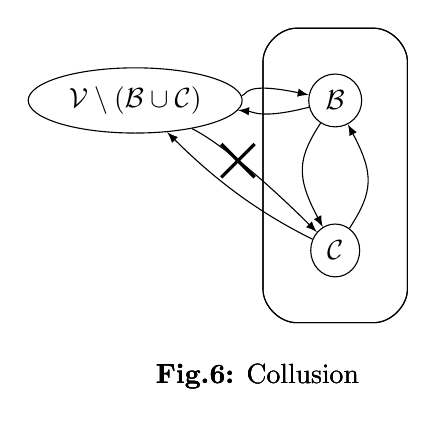
\begin{tikzpicture}[>=latex,line join=bevel,]
%%
\begin{scope}
  \definecolor{strokecol}{rgb}{0.0,0.0,0.0};
  \pgfsetstrokecolor{strokecol}
  \draw (62.0bp,11.5bp) node {\textbf{Fig.6:} Collusion};
\end{scope}
\begin{scope}
  \pgfsetstrokecolor{black}
  \definecolor{strokecol}{rgb}{0.0,0.0,0.0};
  \pgfsetstrokecolor{strokecol}
  \draw (76.0bp,31.0bp) .. controls (76.0bp,31.0bp) and (104.0bp,31.0bp)  .. (104.0bp,31.0bp) .. controls (110.0bp,31.0bp) and (116.0bp,37.0bp)  .. (116.0bp,43.0bp) .. controls (116.0bp,43.0bp) and (116.0bp,125.0bp)  .. (116.0bp,125.0bp) .. controls (116.0bp,131.0bp) and (110.0bp,137.0bp)  .. (104.0bp,137.0bp) .. controls (104.0bp,137.0bp) and (76.0bp,137.0bp)  .. (76.0bp,137.0bp) .. controls (70.0bp,137.0bp) and (64.0bp,131.0bp)  .. (64.0bp,125.0bp) .. controls (64.0bp,125.0bp) and (64.0bp,43.0bp)  .. (64.0bp,43.0bp) .. controls (64.0bp,37.0bp) and (70.0bp,31.0bp)  .. (76.0bp,31.0bp);
  \draw (62.0bp,11.5bp) node {\textbf{Fig.6:} Collusion};
\end{scope}
\begin{scope}
  \pgfsetstrokecolor{black}
  \definecolor{strokecol}{rgb}{0.0,0.0,0.0};
  \pgfsetstrokecolor{strokecol}
  \draw (76.0bp,31.0bp) .. controls (76.0bp,31.0bp) and (104.0bp,31.0bp)  .. (104.0bp,31.0bp) .. controls (110.0bp,31.0bp) and (116.0bp,37.0bp)  .. (116.0bp,43.0bp) .. controls (116.0bp,43.0bp) and (116.0bp,125.0bp)  .. (116.0bp,125.0bp) .. controls (116.0bp,131.0bp) and (110.0bp,137.0bp)  .. (104.0bp,137.0bp) .. controls (104.0bp,137.0bp) and (76.0bp,137.0bp)  .. (76.0bp,137.0bp) .. controls (70.0bp,137.0bp) and (64.0bp,131.0bp)  .. (64.0bp,125.0bp) .. controls (64.0bp,125.0bp) and (64.0bp,43.0bp)  .. (64.0bp,43.0bp) .. controls (64.0bp,37.0bp) and (70.0bp,31.0bp)  .. (76.0bp,31.0bp);
  \draw (62.0bp,11.5bp) node {\textbf{Fig.6:} Collusion};
\end{scope}
  \node (C) at (90.0bp,57.0bp) [draw,ellipse] {$\mathcal{C}$};
  \node (B) at (90.0bp,111.0bp) [draw,ellipse] {$\mathcal{B}$};
  \node (V) at (18.0bp,111.0bp) [draw,ellipse] {$\mathcal{V} \setminus \left(\mathcal{B} \cup \mathcal{C}\right)$};
  \draw [->] (B) ..controls (76.448bp,90.029bp) and (75.776bp,83.771bp)  .. (C);
  \draw [->] (B) ..controls (63.4bp,104.15bp) and (60.49bp,106.97bp)  .. (V);
  \draw [->] (V) ..controls (46.585bp,96.812bp) and (62.033bp,84.876bp)  .. (C);
  \draw (61bp,95.322bp) -- (49bp,83.322bp) [very thick];
  \draw (61bp,83.322bp) -- (49bp,95.322bp) [very thick];
  \draw [->] (C) ..controls (61.68bp,70.995bp) and (46.317bp,82.847bp)  .. (V);
  \draw [->] (V) ..controls (58.496bp,112.85bp) and (56.403bp,118.03bp)  .. (B);
  \draw [->] (C) ..controls (103.56bp,78.024bp) and (104.22bp,84.282bp)  .. (B);
%
\end{tikzpicture}
    \end{center}
    \begin{theorem}[Sybil Resilience] \ \\
       \label{sybil}
       Let $\mathcal{G}$ be a game graph and $\left(\mathcal{B}, \mathcal{C}\right)$ be a collusion of players on
       $\mathcal{G}$. It is
       \begin{equation*}
          Tr_{A \rightarrow \mathcal{B} \cup \mathcal{C}} = Tr_{A \rightarrow \mathcal{B}} \enspace.
       \end{equation*}
    \end{theorem}
    \begin{proofsketch}
       The incoming trust to $\mathcal{B} \cup \mathcal{C}$ cannot be higher than the incoming trust to $\mathcal{B}$ since
       $\mathcal{C}$ has no incoming trust from $\mathcal{V} \setminus \left(\mathcal{B} \cup \mathcal{C}\right)$.%players outside the collusion.
%       For the complete proof, see the Appendix (proof \ref{sybilproof}).
    \end{proofsketch}
    We have proven that controlling $|\mathcal{C}|$ is irrelevant for Eve, thus Sybil attacks are meaningless.

    We have successfully delivered our promise for a Sybil-resilient decentralized financial trust system with
    invariant risk for purchases.

  \section{Related Work}
     The topic of trust has been repeatedly attacked with several approaches: Purely cryptographic infrastructure where trust
     is rather binary and transitivity is not possible is explored in PGP \cite{pgp}. A transitive web-of-trust for fighting
     spam is explored in Freenet \cite{freenet}. Other systems require central trusted
     third parties, such as PKI \cite{pki} and Bazaar \cite{bazaar}, or, in the case of BFT, authenticated membership
     \cite{byzantine}. While other trust systems attempt to be decentralized, they do not prove any Sybil resilience
     properties and hence may be Sybil attackable. Such systems are FIRE \cite{fire}, CORE \cite{core} and others
     \cite{openrep,ghkkw,rk}. Other systems that define trust in a non-financial way are
     \cite{mui,beta,pace,vpc,sdt,wot,pathfinder}.

     The Beaver marketplace \cite{beaver} includes a trust model that relies on
     fees to discourage Sybil attacks. We chose to avoid fees in our system and mitigate Sybil attacks in a different manner.
     Our motivating application for exploring trust in a decentralized setting is the OpenBazaar marketplace. Transitive
     financial trust for OpenBazaar has previously been explored by \cite{dionyziz}. That work however does not define trust
     as a monetary value. We are strongly inspired by \cite{kmrs}
     which gives a sociological justification for the central design choice of identifying trust with
     risk. We greatly appreciate the work in TrustDavis \cite{davis}, which proposes a financial trust system that exhibits
     transitive properties and in which trust is defined as lines-of-credit, similar to our system. We were able to extend
     their work by using the blockchain for automated proofs-of-risk, a feature not available to them at the time. Our
     conservative strategy and the Transitive Game are very similar to the mechanism proposed by the economic paper
     \cite{iou} which also illustrates financial trust transitivity. 

  \section{Further Research}

     %\subsection{Trust Transfer Algorithms}
        When $Alice$ makes a purchase from $Bob$, she has to reduce her outgoing direct trust in a manner such that the
        supposition (\ref{primetrust}) of Risk Invariance theorem is satisfied. How $Alice$ can recalculate her outgoing
        trust will be discussed in a future paper.

     %\subsection{Dynamic Setting}
        Our game is static. In a future dynamic setting, users should be able to play simultaneously, freely join, depart or
        disconnect temporarily from the network. Other types of multisigs, such as 1-of-3, can be explored for the
        implementation of multi-party trust.

     %\subsection{Zero knowledge}
        MaxFlow in our case needs complete network knowledge, which can lead to privacy issues through deanonymisation
        techniques \cite{deanonymisation}. Calculating the flows in zero knowledge remains an open question.

     %\subsection{Game Theoretic Analysis}
        Our game theoretic analysis is simple. An interesting analysis would involve modelling repeated purchases with the
        respective edge updates on the trust graph and treating trust on the network as part of the utility function.

     %\subsection{Implementation and Experimental Results}
        An implementation as a wallet on any blockchain of our financial game is most welcome. A simulation or actual
        implementation of TrustIsRisk, combined with analysis of the resulting dynamics can yield interesting experimental
        results. Subsequently, our trust network can be used in other applications, such as decentralized social networks
        \cite{synereo}.

  \section*{Appendix}
    \subsection{Common Notation}
     \begin{definition}[Neighbourhood]
        \label{neighbourhood}
        \begin{enumerate}
           \item Let $N^{+}\left(A\right)_j$ be the set of players $B$ that $A$ directly trusts with any positive value at
              the end of turn $j$. More formally,
              \begin{equation}
                 N^{+}\left(A\right)_j = \{B \in \mathcal{V}_j : DTr_{A \rightarrow B, j} > 0\} \enspace.
              \end{equation}
              $N^{+}\left(A\right)_j$ is called out neighbourhood of $A$ on turn $j$. Let $S \subseteq \mathcal{V}_j$. Then
              \begin{equation}
                 N^{+}\left(S\right)_j = \bigcup\limits_{A \in S}N^{+}\left(A\right)_j \enspace.
              \end{equation}
           \item Let $N^{-}\left(A\right)_j$ be the set of players $B$ that directly trust $A$ with any positive value at the
              end of turn $j$. More formally,
              \begin{equation}
                 N^{-}\left(A\right)_j = \{B \in \mathcal{V}_j : DTr_{B \rightarrow A, j} > 0\} \enspace.
              \end{equation}
              $N^{-}\left(A\right)_j$ is called in neighbourhood of $A$ on turn $j$. Let $S \subseteq \mathcal{V}_j$. Then
              \begin{equation}
                 N^{-}\left(S\right)_j = \bigcup\limits_{A \in S}N^{-}\left(A\right)_j \enspace.
              \end{equation}
           \item Let $N\left(A\right)_j$ be the set of players $B$ that either directly trust or are directly trusted by $A$
              with any positive value at the end of turn $j$. More formally,
              \begin{equation}
                 N\left(A\right)_j = N^{+}\left(A\right)_j \cup N^{-}\left(A\right)_j \enspace.
              \end{equation}
              $N\left(A\right)_j$ is called neighbourhood of $A$ on turn $j$. Let $S \subset \mathcal{V}_j$. Then
              \begin{equation}
                 N\left(S\right)_j = N^{+}\left(S\right)_j \cup N^{-}\left(S\right)_j \enspace.
              \end{equation}
        \end{enumerate}
     \end{definition}
     \begin{definition}[Total Incoming/Outgoing Trust]
     \label{inouttrust}
        \begin{equation}
           in_{A, j} = \sum\limits_{v \in N^{-}\left(A\right)_j}DTr_{v \rightarrow A, j}
        \end{equation}
        \begin{equation}
           out_{A, j} = \sum\limits_{v \in N^{+}\left(A\right)_j}DTr_{A \rightarrow v, j}
        \end{equation}
     \end{definition}
     \newpage 
     Here we add some concrete $Turn_j$ examples. Let $A = Player(j)$.
     \begin{enumerate}
        \item \begin{equation*}
           Turn_j = \emptyset
        \end{equation*}
        \item \begin{equation*}
           Turn_j = \{Steal\left(y, B\right), Add\left(w, B\right)\} \enspace,
        \end{equation*}
        given that
        \begin{equation*}
           0 \leq y \leq DTr_{B \rightarrow A, j-1} \wedge -DTr_{A \rightarrow B, j-1} \leq w \wedge w - y \leq
           Cap_{A, j-1} \enspace.
        \end{equation*}
        \item \begin{equation*}
           Turn_j = \{Steal\left(x, B\right), Add\left(y, C\right), Add\left(w, D\right)\} \enspace,
        \end{equation*}
        given that
        \begin{equation*}
        \begin{gathered}
           0 \leq x \leq DTr_{B \rightarrow A, j-1} \wedge -DTr_{A \rightarrow C, j-1} \leq y \: \wedge \\
           \wedge -DTr_{A \rightarrow D, j-1} \leq w \wedge y + w - x \leq Cap_{A, j-1} \enspace.
        \end{gathered}
        \end{equation*}
        \item \begin{equation*}
           Turn_j = \{Steal\left(x, B\right), Steal\left(y, B\right)\}
        \end{equation*}
        is not a valid turn because it contains two $Steal\left(\right)$ actions against the same player. If
        \begin{equation*}
           0 \leq x \wedge 0 \leq y \wedge x + y \leq DTr_{B \rightarrow A, j-1} \enspace,
        \end{equation*}
        the correct alternative would be
        \begin{equation*}
           Turn_j = \{Steal\left(x+y, B\right)\} \enspace.
        \end{equation*}
     \end{enumerate}
     \begin{definition}[Previous/Next Turn]
        Let $j \in \mathbb{N}$ a turn with $Player\left(j\right)$ $= A$. We define $prev\left(j\right), next\left(j\right)$
        as the previous and next turn that $A$ is chosen to play respectively. If $j$ is the first turn that $A$ plays,
        $prev\left(j\right) = 0$. More formally, if
        \begin{equation*}
           P = \{k \in \mathbb{N} : k < j \wedge Player\left(k\right) = A\} \mbox{ and}
        \end{equation*}
        \begin{equation*}
           N = \{k \in \mathbb{N} : k > j \wedge Player\left(k\right) = A\} \enspace,
        \end{equation*}
        then we define $prev\left(j\right), next\left(j\right)$ as follows:
        \begin{equation}
           prev\left(j\right) = \begin{cases}
              \max{P}, & P \neq \emptyset \\
              0, & P = \emptyset
           \end{cases}
        \end{equation}
        \begin{equation}
           next\left(j\right) = \min{N}
        \end{equation}
        $next\left(j\right)$ is always well defined with the assumption that after each turn eventually everybody plays.
     \end{definition}
    \subsection{Proofs, Lemmas and Theorems}
    \begin{lemma}[$Loss$ Equivalent to $Damage$] \ \\
       Consider a Transitive Game. Let $j \in \mathbb{N}$ and $v = Player\left(j\right)$ such that $v$ is following the
       conservative strategy. It holds that
       \begin{equation*}
          \min\left(in_{v, j}, Loss_{v, j}\right) = \min\left(in_{v, j}, Damage_{v, j}\right) \enspace.
       \end{equation*}
    \end{lemma}
    \begin{proof} \ \\
          \textbf{Case 1:} Let $v \in Happy_{j-1}$. Then
          \begin{enumerate}
             \item $v \in Happy_j$ because $Turn_{j} = \emptyset$,
             \item $Loss_{v, j} = 0$ because otherwise $v \notin Happy_j$,
             \item $Damage_{v, j} = 0$, or else any reduction in direct trust to $v$ would increase equally
             $Loss_{v, j}$ (line~\ref{trsteallossincrease}), which cannot be decreased again but during an Angry player's turn
             (line~\ref{trsteallossdecrease}).
             \item $in_{v, j} \geq 0$
          \end{enumerate}
          Thus
          \begin{equation*}
             \min\left(in_{v, j}, Loss_{v,j}\right) = \min\left(in_{v, j}, Damage_{v,j}\right) = 0 \enspace.
          \end{equation*}
          \textbf{Case 2:} Let $v \in Sad_{j-1}$. Then
          \begin{enumerate}
             \item $v \in Sad_j$ because $Turn_{j} = \emptyset$, 
             \item $in_{v, j} = 0$ (line~\ref{trstealifentersad}),
             \item $Damage_{v, j} \geq 0 \wedge Loss_{v, j} \geq 0$.
          \end{enumerate}
          Thus
          \begin{equation*}
             \min\left(in_{v, j}, Loss_{v,j}\right) = \min\left(in_{v, j}, Damage_{v,j}\right) = 0 \enspace.
          \end{equation*}
          If $v \in Angry_{j-1}$ then the same argument as in cases 1 and 2 hold when $v \in Happy_j$ and $v \in Sad_j$
          respectively if we ignore the argument (1). Thus the theorem holds in every case.
    \end{proof}

    \begin{sepproof}{Proof of Theorem \ref{convergence}: Trust Convergence} \ \\
    \label{convergenceproof}
       First of all, after turn $j_0$ player $E$ will always pass her turn
       because she has already nullified her incoming and outgoing direct trusts in $Turn_{j_0}$, the evil strategy does not
       contain any case where direct trust is increased or where the evil player starts directly trusting another player and
       the other players do not follow a strategy in which they can choose to $Add\left(\right)$ trust to $E$. The same holds
       for player $A$ because she follows the idle strategy. As far as the rest of the players are concerned, consider the
       Transitive Game. As we can see from lines~\ref{trsteallossinit} and~\ref{trsteallossincrease}
       -~\ref{trsteallossdecrease}, it is
       \begin{equation*}
          \forall j, \sum\limits_{v \in \mathcal{V}_j}Loss_v = in_{E, j_0-1} \enspace.
       \end{equation*}
       In other words, the total loss is constant and equal to the total value stolen by $E$. Also, as we can see in
       lines~\ref{trstealsadinit} and~\ref{trstealtrueentersad}, which are the only lines where the $Sad$ set is modified,
       once a player enters the $Sad$ set, it is impossible to exit from this set. Also, we can see that players in $Sad
       \cup Happy$ always pass their turn. We will now show that eventually the $Angry$ set will be empty, or equivalently
       that eventually every player will pass their turn. Suppose that it is possible to have an infinite amount of turns
       in which players do not choose to pass. We know that the number of nodes is finite, thus this is possible only if
       \begin{equation*}
          \exists j': \forall j \geq j', |Angry_j \cup Happy_j| = c > 0 \wedge Angry_j \neq \emptyset \enspace.
       \end{equation*}
       This statement is valid because the total number of angry and happy players cannot increase because no player leaves
       the $Sad$ set and if it were to be decreased, it would eventually reach 0. Since $Angry_j \neq \emptyset$, a player
       $v$ that will not pass her turn will eventually be chosen to play. According to the Transitive Game, $v$ will either
       deplete her incoming trust and enter the $Sad$ set (line~\ref{trstealtrueentersad}), which is contradicting $|Angry_j
       \cup Happy_j| = c$, or will steal enough value to enter the $Happy$ set, that is $v$ will achieve $Loss_{v, j} = 0$.
       Suppose that she has stolen $m$ players. They, in their turn, will steal total value at least equal to the value
       stolen by $v$ (since they cannot go sad, as explained above). However, this means that, since the total value being
       stolen will never be reduced and the turns this will happen are infinite, the players must steal an infinite amount of
       value, which is impossible because the direct trusts are finite in number and in value. More precisely, let $j_1$ be
       a turn in which a conservative player is chosen and
       \begin{equation*}
          \forall j \in \mathbb{N}, DTr_j = \sum\limits_{w,w' \in \mathcal{V}}DTr_{w \rightarrow w', j} \enspace.
       \end{equation*}
       Also, without loss of generality, suppose that
       \begin{equation*}
          \forall j \geq j_1, out_{A, j} = out_{A, j_1} \enspace.
       \end{equation*}
       In $Turn_{j_1}$, $v$ steals
       \begin{equation*}
          St = \sum\limits_{i=1}^{m}y_i \enspace.
       \end{equation*}
       We will show using induction that
       \begin{equation*}
          \forall n \in \mathbb{N}, \exists j_n \in \mathbb{N} : DTr_{j_n} \leq DTr_{j_1-1} - nSt \enspace.
       \end{equation*}

       Base case: It holds that
       \begin{equation*}
          DTr_{j_1} = DTr_{j_1-1} - St \enspace.
       \end{equation*}
       Eventually there is a turn $j_2$ when every player in $N^{-}(v)_{j-1}$ will have played. Then it holds that
       \begin{equation*}
          DTr_{j_2} \leq DTr_{j_1} - St = DTr_{j_1-1} - 2St \enspace,
       \end{equation*}
       since all players in $N^{-}(v)_{j-1}$ follow the conservative strategy, except for $A$, who will not have been stolen
       anything due to the supposition.

       Induction hypothesis: Suppose that
       \begin{equation*}
          \exists k > 1 : j_k > j_{k-1} > j_1 \Rightarrow DTr_{j_k} \leq DTr_{j_{k-1}} - St \enspace.
       \end{equation*}

       Induction step: There exists a subset of the $Angry$ players, $S$, that have been stolen at least value $St$ in total
       between the turns $j_{k-1}$ and $j_k$, thus there exists a turn $j_{k+1}$ such that all players in $S$ will have
       played and thus
       \begin{equation*}
          DTr_{j_{k+1}} \leq DTr_{j_k} - St \enspace.
       \end{equation*}
       We have proven by induction that
       \begin{equation*}
          \forall n \in \mathbb{N}, \exists j_n \in \mathbb{N} : DTr_{j_n} \leq DTr_{j_1-1} - nSt \enspace.
       \end{equation*}
       However
       \begin{equation*}
          DTr_{j_1-1} \geq 0 \wedge St > 0 \enspace,
       \end{equation*}
       thus
       \begin{equation*}
          \exists n' \in \mathbb{N} : n'St > DTr_{j_1-1} \Rightarrow DTr_{j_{n'}} < 0 \enspace.
       \end{equation*}
       We have a contradiction because
       \begin{equation*}
          \forall w,w' \in \mathcal{V}, \forall j \in \mathbb{N}, DTr_{w \rightarrow w', j} \geq 0 \enspace,
       \end{equation*}
       thus eventually $Angry = \emptyset$ and everybody passes. \qed
    \end{sepproof}

    \begin{sepproof}{Proof of Lemma \ref{maxflowgame}: MaxFlows Are Transitive Games} \ \\
    \label{maxflowgameproof}
       We suppose that the turn of $\mathcal{G}$ is 0. In other words, $\mathcal{G} = \mathcal{G}_0$. Let
       $X = \{x_{vw}\}_{\mathcal{V} \times \mathcal{V}}$ be the flows returned by $MaxFlow\left(A, E\right)$. For any graph
       $G$ there exists a $MaxFlow$ that is a DAG. We can easily prove this using the Flow Decomposition theorem
       \cite{amo}, which states that each flow can be seen as a finite set of paths from $A$ to $E$ and cycles, each
       having a certain flow. We execute $MaxFlow\left(A, E\right)$ and we apply the aforementioned theorem. The
       cycles do not influence the $maxFlow\left(A, E\right)$, thus we can remove these flows. The resulting flow is a
       $MaxFlow\left(A, E\right)$ without cycles, thus it is a DAG. Topologically sorting this DAG, we obtain a total order
       of its nodes such that $\forall$ nodes $v, w \in \mathcal{V} : v < w \Rightarrow x_{wv} = 0$ \cite{clrs}. Put
       differently, there is no flow from larger to smaller nodes. $E$ is maximum since it is the sink and thus has no
       outgoing flow to any node and $A$ is minimum since it is the source and thus has no incoming flow from any node. The
       desired execution of Transitive Game will choose players following the total order inversely, starting from player
       $E$. We observe that $\forall v \in \mathcal{V} \setminus \{A, E\}, \sum\limits_{w \in \mathcal{V}}x_{wv} =
       \sum\limits_{w \in \mathcal{V}}x_{vw} \leq maxFlow\left(A, E\right) \leq in_{E, 0}$. Player $E$ will follow a modified
       evil strategy where she steals value equal to her total incoming flow, not her total incoming trust. Let $j_2$ be the
       first turn when $A$ is chosen to play. We will show using strong induction that there exists a set of valid actions
       for each player according to their respective strategy such that at the end of each turn $j$ the corresponding player
       $v = Player\left(j\right)$ will have stolen value $x_{wv}$ from each in-neighbour $w$.

       Base case: In turn 1, $E$ steals value equal to $\sum\limits_{w \in \mathcal{V}}x_{wE}$, following the modified evil
       strategy.
       \begin{equation*}
          Turn_1 = \bigcup\limits_{v \in N^{-}\left(E\right)_0}\{Steal\left(x_{vE}, v\right)\}
       \end{equation*}

       Induction hypothesis: Let $k \in [j_2 - 2]$. We suppose that $\forall i \in [k]$, there exists a valid set of actions,
       $Turn_i$, performed by $v = Player\left(i\right)$ such that $v$ steals from each player $w$ value equal to $x_{wv}$.
       \begin{equation*}
          \forall i \in [k], Turn_i = \bigcup\limits_{w \in N^{-}\left(v\right)_{i-1}}\{Steal\left(x_{wv}, w\right)\}
       \end{equation*}

       Induction step: Let $j = k + 1, v = Player\left(j\right)$. Since all the players that are greater than $v$ in the
       total order have already played and all of them have stolen value equal to their incoming flow, we deduce that $v$ has
       been stolen value equal to $\sum\limits_{w \in N^{+}\left(v\right)_{j-1}}x_{vw}$. Since it is the first time $v$
       plays, $\forall w \in N^{-}\left(v\right)_{j-1}, DTr_{w \rightarrow v, j-1} = DTr_{w \rightarrow v, 0} \geq x_{wv}$, thus
       $v$ is able to choose the following turn:
       \begin{equation*}
          Turn_j = \bigcup\limits_{w \in N^{-}\left(v\right)_{j-1}}\{Steal\left(x_{wv}, w\right)\}
       \end{equation*}
       Moreover, this turn satisfies the conservative strategy since
       \begin{equation*}
          \sum\limits_{w \in N^{-}\left(v\right)_{j-1}}x_{wv} = \sum\limits_{w \in N^{+}\left(v\right)_{j-1}}x_{vw} \enspace.
       \end{equation*}
       Thus $Turn_j$ is a valid turn for the conservative player $v$.

       We have proven that in the end of turn $j_2 - 1$, player $E$ and all the conservative players will have stolen value
       exactly equal to their total incoming flow, thus $A$ will have been stolen value equal to her outgoing flow, which is
       $maxFlow(A, E)$. Since there remains no Angry player, $j_2$ is a convergence turn, thus $Loss_{A, j_2} = Loss_A$. We
       can also see that if $E$ had chosen the original evil strategy, the described actions would still be valid only by
       supplementing them with additional $Steal\left(\right)$ actions, thus $Loss_A$ would further increase. This proves the
       theorem. \qed
    \end{sepproof}

    \begin{sepproof}{Proof of Lemma \ref{gameflow}: Transitive Games Are Flows} \ \\
    \label{gameflowproof}
       Let $Sad, Happy, Angry$ be as defined in the Transitive Game. Let $\mathcal{G}'$ be a directed weighted graph based on
       $\mathcal{G}$ with an auxiliary source. Let also $j_1$ be a turn when the Transitive Game has converged. More
       precisely, $\mathcal{G}'$ is defined as follows:
       \begin{equation*}
          \mathcal{V}' = \mathcal{V} \cup \{T\}
       \end{equation*}
       \begin{equation*}
          \mathcal{E}' = \mathcal{E} \cup \{(T, A)\} \cup \{(T, v) : v \in Sad_{j_1}\}
       \end{equation*}
       \begin{equation*}
          \forall (v, w) \in \mathcal{E}, c'_{vw} = DTr_{v \rightarrow w, 0} - DTr_{v \rightarrow w, j_1}
       \end{equation*}
       \begin{equation*}
          \forall v \in Sad_{j_1}, c'_{Tv} = c'_{TA} = \infty
       \end{equation*}
       \begin{center}
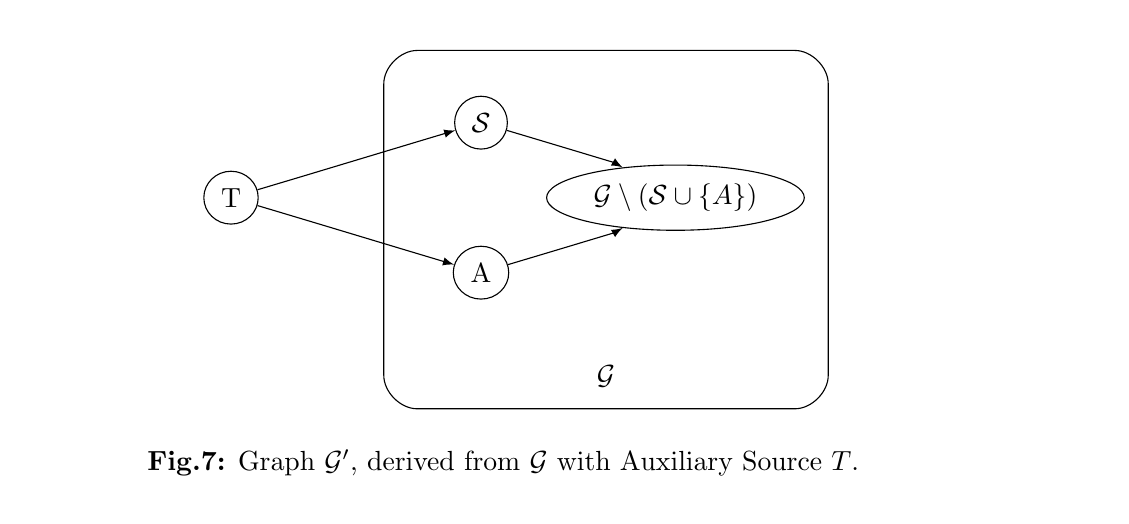
\begin{tikzpicture}[>=latex,line join=bevel,]
%%
\begin{scope}
  \definecolor{strokecol}{rgb}{0.0,0.0,0.0};
  \pgfsetstrokecolor{strokecol}
  \draw (171.0bp,11.5bp) node {\textbf{Fig.7:} Graph $\mathcal{G}'$, derived from $\mathcal{G}$ with Auxiliary Source $T$.};
\end{scope}
\begin{scope}
  \pgfsetstrokecolor{black}
  \definecolor{strokecol}{rgb}{1.0,1.0,1.0};
  \pgfsetstrokecolor{strokecol}
  \definecolor{fillcol}{rgb}{1.0,1.0,1.0};
  \pgfsetfillcolor{fillcol}
  \filldraw (0.0bp,0.0bp) -- (0.0bp,168.0bp) -- (386.0bp,168.0bp) -- (386.0bp,0.0bp) -- cycle;
  \definecolor{strokecol}{rgb}{0.0,0.0,0.0};
  \pgfsetstrokecolor{strokecol}
  \draw (171.0bp,11.5bp) node {\textbf{Fig.7:} Graph $\mathcal{G}'$, derived from $\mathcal{G}$ with Auxiliary Source $T$.};
\end{scope}
\begin{scope}
  \pgfsetstrokecolor{black}
  \definecolor{strokecol}{rgb}{0.0,0.0,0.0};
  \pgfsetstrokecolor{strokecol}
  \draw (140.0bp,31.0bp) .. controls (140.0bp,31.0bp) and (276.0bp,31.0bp)  .. (276.0bp,31.0bp) .. controls (282.0bp,31.0bp) and (288.0bp,37.0bp)  .. (288.0bp,43.0bp) .. controls (288.0bp,43.0bp) and (288.0bp,148.0bp)  .. (288.0bp,148.0bp) .. controls (288.0bp,154.0bp) and (282.0bp,160.0bp)  .. (276.0bp,160.0bp) .. controls (276.0bp,160.0bp) and (140.0bp,160.0bp)  .. (140.0bp,160.0bp) .. controls (134.0bp,160.0bp) and (128.0bp,154.0bp)  .. (128.0bp,148.0bp) .. controls (128.0bp,148.0bp) and (128.0bp,43.0bp)  .. (128.0bp,43.0bp) .. controls (128.0bp,37.0bp) and (134.0bp,31.0bp)  .. (140.0bp,31.0bp);
  \draw (208.0bp,42.5bp) node {$\mathcal{G}$};
\end{scope}
  \node (A) at (163.0bp,80.0bp) [draw,ellipse] {A};
  \node (S) at (163.0bp,134.0bp) [draw,ellipse] {$\mathcal{S}$};
  \node (T) at (73.0bp,107.0bp) [draw,ellipse] {T};
  \node (G) at (233.0bp,107.0bp) [draw,ellipse] {$\mathcal{G} \setminus \left(\mathcal{S} \cup \{A\}\right)$};
  \draw [->] (A) ..controls (198.61bp,90.619bp) and (211.12bp,94.457bp)  .. (G);
  \draw [->] (S) ..controls (198.61bp,123.38bp) and (211.12bp,119.54bp)  .. (G);
  \draw [->] (T) ..controls (108.61bp,117.62bp) and (121.12bp,121.46bp)  .. (S);
  \draw [->] (T) ..controls (108.61bp,96.381bp) and (121.12bp,92.543bp)  .. (A);
%
\end{tikzpicture}
       \end{center}
       In the figure above, $\mathcal{S}$ is the set of sad players. We observe that $\forall v \in \mathcal{V},$
       \begin{equation}
       \label{gameflowin}
       \begin{gathered}
          \sum\limits_{w \in N^{-}\left(v\right)' \setminus \{T\}}c'_{wv} = \\
          = \sum\limits_{w \in N^{-}\left(v\right)' \setminus \{T\}}\left(DTr_{w \rightarrow v, 0} -
          DTr_{w \rightarrow v, j_1}\right) = \\
          = \sum\limits_{w \in N^{-}\left(v\right)' \setminus \{T\}}DTr_{w \rightarrow v, 0} -
          \sum\limits_{w \in N^{-}\left(v\right)' \setminus \{T\}}DTr_{w \rightarrow v, j-1} =  \\
          = in_{v, 0} - in_{v, j_1}
       \end{gathered}
       \end{equation}
       and
       \begin{equation}
       \label{gameflowout}
       \begin{gathered}
          \sum\limits_{w \in N^{+}\left(v\right)' \setminus \{T\}}c'_{vw} = \\
          = \sum\limits_{w \in N^{+}\left(v\right)' \setminus \{T\}}\left(DTr_{v \rightarrow w, 0} -
          DTr_{v \rightarrow w, j_1}\right) = \\
          = \sum\limits_{w \in N^{+}\left(v\right)' \setminus \{T\}}DTr_{v \rightarrow w, 0} -
          \sum\limits_{w \in N^{+}\left(v\right)' \setminus \{T\}}DTr_{v \rightarrow w, j-1} = \\
          = out_{v, 0} - out_{v, j_1} \enspace.
       \end{gathered}
       \end{equation}
       We can suppose that
       \begin{equation}
       \label{Aincoming}
          \forall j \in \mathbb{N}, in_{A, j} = 0 \enspace,
       \end{equation}
       since if we find a valid flow under this assumption, the flow will still be valid for the original graph. \\
       Next we try to calculate $MaxFlow\left(T, E\right) = X'$ on graph $\mathcal{G}'$. We observe that a flow in which it
       holds that $\forall v, w \in \mathcal{V}, x'_{vw} = c'_{vw}$ can be valid for the following reasons:
       \begin{itemize}
          \item $\forall v,w \in \mathcal{V}, x'_{vw} \leq c'_{vw}$ (Capacity flow requirement (\ref{flow1}) $\forall e \in
          \mathcal{E}$)
          \item Since $\forall v \in Sad_{j_1} \cup \{A\}, c'_{Tv} = \infty$, requirement (\ref{flow1}) holds for any flow
          $x'_{Tv} \geq 0$.
          \item Let $v \in \mathcal{V}' \setminus \left(Sad_{j_1} \cup \{T, A, E\}\right)$. According to the conservative
          strategy and since $v \notin Sad_{j_1},$ it holds that
          \begin{equation*}
             out_{v, 0} - out_{v, j_1} = in_{v, 0} - in_{v, j_1} \enspace.
          \end{equation*}
          Combining this observation with (\ref{gameflowin}) and (\ref{gameflowout}), we have that
          \begin{equation*}
             \sum\limits_{w \in \mathcal{V}'}c'_{vw} = \sum\limits_{w \in \mathcal{V}'}c'_{wv} \enspace.
          \end{equation*}
          (Flow Conservation requirement (\ref{flow2}) $\forall v \in \mathcal{V}' \setminus \left(Sad_{j_1}
          \cup \{T, A, E\}\right)$)
          \item Let $v \in Sad_{j_1}$. Since $v$ is sad, we know that
          \begin{equation*}
             out_{v, 0} - out_{v, j_1} > in_{v, 0} - in_{v, j_1} \enspace.
          \end{equation*}
          Since $c'_{Tv} = \infty$, we can set
          \begin{equation*}
             x'_{Tv} = \left(out_{v, 0} - out_{v, j_1}\right) - \left(in_{v, 0} - in_{v, j_1}\right) \enspace.
          \end{equation*}
          In this way, we have
          \begin{equation*}
             \sum\limits_{w \in \mathcal{V}'}x'_{vw} = out_{v, 0} - out_{v, j_1} \mbox{ and}
          \end{equation*}
          \begin{equation*}
          \begin{gathered}
             \sum\limits_{w \in \mathcal{V}'}x'_{wv} = \sum\limits_{w \in \mathcal{V}' \setminus \{T\}}c'_{wv} + x'_{Tv} =
             in_{v, 0} - in_{v, j_1} + \\ + (out_{v, 0} - out_{v, j_1}) - (in_{v, 0} - in_{v, j_1}) = out_{v, 0} -
             out_{v, j_1} \enspace.
          \end{gathered}
          \end{equation*}
          thus
          \begin{equation*}
             \sum\limits_{w \in \mathcal{V}'}x'_{vw} = \sum\limits_{w \in \mathcal{V}'}x'_{wv} \enspace.
          \end{equation*}
          (Requirement \ref{flow2} $\forall v \in Sad_{j_1}$)
          \item We set
          \begin{equation*}
             x'_{TA} = \sum\limits_{v \in \mathcal{V}'}x'_{Av} \enspace,
          \end{equation*}
          thus from (\ref{Aincoming}) we have
          \begin{equation*}
             \sum\limits_{v \in \mathcal{V}'}x'_{vA} = \sum\limits_{v \in \mathcal{V}'}x'_{Av} \enspace.
          \end{equation*}
          (Requirement \ref{flow2} for $A$)
       \end{itemize}
       We saw that for all nodes, the necessary properties for a flow to be valid hold and thus $X'$ is a valid flow for
       $\mathcal{G}$. Moreover, this flow is equal to $maxFlow(T, E)$ because all incoming flows to $E$ are saturated.
       Also we observe that
       \begin{equation}
       \label{xprimeequalloss}
          \sum\limits_{v \in \mathcal{V}'}x'_{Av} = \sum\limits_{v \in \mathcal{V}'}c'_{Av} = out_{A, 0} - out_{A, j_1} =
          Loss_A \enspace.
       \end{equation}
       We define another graph, $\mathcal{G}''$, based on $\mathcal{G}'$.
       \begin{equation*}
          \mathcal{V}'' = \mathcal{V}'
       \end{equation*}
       \begin{equation*}
          E(\mathcal{G}'') = E(\mathcal{G}') \setminus \{(T, v) : v \in Sad_j\}
       \end{equation*}
       \begin{equation*}
          \forall e \in E(\mathcal{G}''), c''_e = c'_e
       \end{equation*}
       If we execute the algorithm $MaxFlow(T, E)$ on the graph $\mathcal{G}''$, we will obtain a flow $X''$ in which
       \begin{equation*}
          \sum\limits_{v \in \mathcal{V}''}x''_{Tv} = x''_{TA} = \sum\limits_{v \in \mathcal{V}''}x''_{Av} \enspace.
       \end{equation*}
       The outgoing flow from $A$ in $X''$ will remain the same as in $X'$ for two reasons: Firstly, using the Flow
       Decomposition theorem \cite{amo} and deleting the paths that contain edges $\left(T, v\right): v \neq A$, we
       obtain a flow configuration where the total outgoing flow from $A$ remains invariant,
%       \footnote{We thank Kyriakos Axiotis for his insights on the Flow Decomposition theorem.}
       thus
       \begin{equation*}
          \sum\limits_{v \in \mathcal{V}''}x''_{Av} \geq \sum\limits_{v \in \mathcal{V}'}x'_{Av} \enspace.
       \end{equation*}
       Secondly, we have
       \begin{equation*}
          \begin{rcases}
             \sum\limits_{v \in \mathcal{V}''}c''_{Av} = \sum\limits_{v \in \mathcal{V}'}c'_{Av} = \sum\limits_{v \in
             \mathcal{V}'}x'_{Av} \\
             \sum\limits_{v \in \mathcal{V}''}c''_{Av} \geq \sum\limits_{v \in \mathcal{V}''}x''_{Av}
          \end{rcases}
          \Rightarrow \sum\limits_{v \in \mathcal{V}''}x''_{Av} \leq \sum\limits_{v \in \mathcal{V}'}x'_{Av} \enspace.
       \end{equation*}
       Thus we conclude that
       \begin{equation}
       \label{primeequaldoubleprime}
          \sum\limits_{v \in \mathcal{V}''}x''_{Av} = \sum\limits_{v \in \mathcal{V}'}x'_{Av} \enspace.
       \end{equation}
       Let $X = X'' \setminus \{(T, A)\}$. Observe that
       \begin{equation*}
          \sum\limits_{v \in \mathcal{V}''}x''_{Av} = \sum\limits_{v \in \mathcal{V}}x_{Av} \enspace.
       \end{equation*}
       This flow is valid on graph $\mathcal{G}$ because
       \begin{equation*}
          \forall e \in \mathcal{E}, c_e \geq c''_e \enspace.
       \end{equation*}
       Thus there exists a valid flow for each execution of the Transitive Game such that
       \begin{equation*}
          \sum\limits_{v \in \mathcal{V}}x_{Av} = \sum\limits_{v \in \mathcal{V}''}x''_{Av}
          \overset{\left(\ref{primeequaldoubleprime}\right)}{=} \sum\limits_{v \in \mathcal{V}'}x'_{Av}
          \overset{\left(\ref{xprimeequalloss}\right)}{=} Loss_{A, j_1} \enspace,
       \end{equation*}
       which is the flow $X$. \qed
    \end{sepproof}

    \begin{theorem}[Conservative World Theorem] \ \\
       \label{conservativeworld}
       If everybody follows the conservative strategy, nobody steals any amount from anybody.
    \end{theorem}
     \begin{proof}
        Let $\mathcal{H}$ be the game history where all players are conservative and suppose there are some
        $Steal\left(\right)$ actions taking place. Then let $\mathcal{H}'$ be the subsequence of turns each containing at
        least one $Steal\left(\right)$ action. This subsequence is evidently nonempty, thus it must have a first element. The
        player corresponding to that turn, $A$, has chosen a $Steal\left(\right)$ action and no previous player has chosen
        such an action. However, player $A$ follows the conservative strategy, which is a contradiction.
     \end{proof}

    \begin{sepproof}{Proof of Theorem \ref{sybil}: Sybil Resilience} \ \\
    \label{sybilproof}
       Let $\mathcal{G}_1$ be a game graph defined as follows:
       \begin{equation*}
          \mathcal{V}_1 = \mathcal{V} \cup \{T_1\} \enspace,
       \end{equation*}
       \begin{equation*}
          \mathcal{E}_1 = \mathcal{E} \cup \{(v, T_1) : v \in \mathcal{B} \cup \mathcal{C}\} \enspace,
       \end{equation*}
       \begin{equation*}
          \forall v,w \in \mathcal{V}_1 \setminus \{T_1\}, DTr^1_{v \rightarrow w} = DTr_{v \rightarrow w} \enspace,
       \end{equation*}
       \begin{equation*}
          \forall v \in \mathcal{B} \cup \mathcal{C}, DTr^1_{v \rightarrow T_1} = \infty \enspace,
       \end{equation*}
       where $DTr_{v \rightarrow w}$ is the direct trust from $v$ to $w$ in $\mathcal{G}$ and $DTr^1_{v \rightarrow w}$ is
       the direct trust from $v$ to $w$ in $\mathcal{G}_1$. \\
       Let also $\mathcal{G}_2$ be the induced graph that results from $\mathcal{G}_1$ if we remove the Sybil set,
       $\mathcal{C}$. We rename $T_1$ to $T_2$ and define $\mathcal{L} = \mathcal{V} \setminus \left(\mathcal{B} \cup
       \mathcal{C}\right)$ as the set of legitimate players to facilitate comprehension.
       \begin{center}
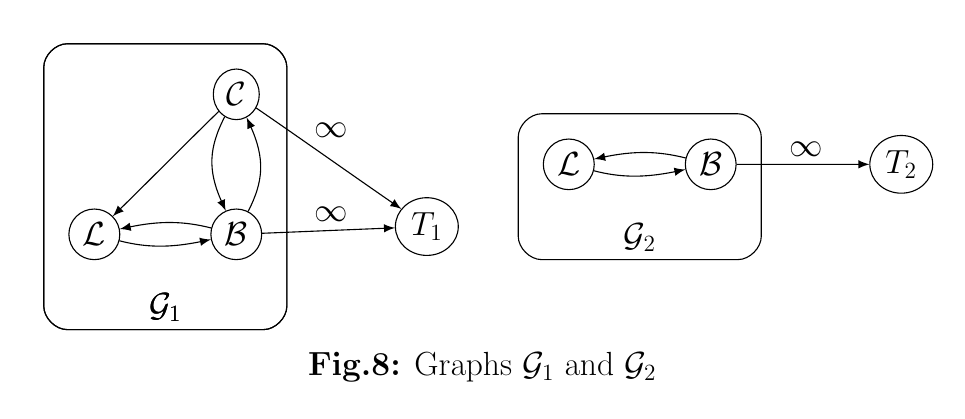
\begin{tikzpicture}[>=latex,line join=bevel,scale=0.7,transform shape]
%%
\begin{scope}
  \definecolor{strokecol}{rgb}{0.0,0.0,0.0};
  \pgfsetstrokecolor{strokecol}
  \draw (233.5bp,11.5bp) node {\LARGE \textbf{Fig.8:} Graphs $\mathcal{G}_1$ and $\mathcal{G}_2$};
\end{scope}
\begin{scope}
  \pgfsetstrokecolor{black}
  \definecolor{strokecol}{rgb}{1.0,1.0,1.0};
  \pgfsetstrokecolor{strokecol}
  \definecolor{fillcol}{rgb}{1.0,1.0,1.0};
  \pgfsetfillcolor{fillcol}
  \filldraw (0.0bp,0.0bp) -- (0.0bp,186.0bp) -- (467.0bp,186.0bp) -- (467.0bp,0.0bp) -- cycle;
  \definecolor{strokecol}{rgb}{0.0,0.0,0.0};
  \pgfsetstrokecolor{strokecol}
  \draw (233.5bp,11.5bp) node {\LARGE \textbf{Fig.8:} Graphs $\mathcal{G}_1$ and $\mathcal{G}_2$};
\end{scope}
\begin{scope}
  \pgfsetstrokecolor{black}
  \definecolor{strokecol}{rgb}{0.0,0.0,0.0};
  \pgfsetstrokecolor{strokecol}
  \draw (20.0bp,31.0bp) .. controls (20.0bp,31.0bp) and (121.0bp,31.0bp)  .. (121.0bp,31.0bp) .. controls (127.0bp,31.0bp) and (133.0bp,37.0bp)  .. (133.0bp,43.0bp) .. controls (133.0bp,43.0bp) and (133.0bp,166.0bp)  .. (133.0bp,166.0bp) .. controls (133.0bp,172.0bp) and (127.0bp,178.0bp)  .. (121.0bp,178.0bp) .. controls (121.0bp,178.0bp) and (20.0bp,178.0bp)  .. (20.0bp,178.0bp) .. controls (14.0bp,178.0bp) and (8.0bp,172.0bp)  .. (8.0bp,166.0bp) .. controls (8.0bp,166.0bp) and (8.0bp,43.0bp)  .. (8.0bp,43.0bp) .. controls (8.0bp,37.0bp) and (14.0bp,31.0bp)  .. (20.0bp,31.0bp);
  \draw (70.5bp,42.5bp) node {\LARGE $\mathcal{G}_1$};
\end{scope}
\begin{scope}
  \pgfsetstrokecolor{black}
  \definecolor{strokecol}{rgb}{0.0,0.0,0.0};
  \pgfsetstrokecolor{strokecol}
  \draw (20.0bp,31.0bp) .. controls (20.0bp,31.0bp) and (121.0bp,31.0bp)  .. (121.0bp,31.0bp) .. controls (127.0bp,31.0bp) and (133.0bp,37.0bp)  .. (133.0bp,43.0bp) .. controls (133.0bp,43.0bp) and (133.0bp,166.0bp)  .. (133.0bp,166.0bp) .. controls (133.0bp,172.0bp) and (127.0bp,178.0bp)  .. (121.0bp,178.0bp) .. controls (121.0bp,178.0bp) and (20.0bp,178.0bp)  .. (20.0bp,178.0bp) .. controls (14.0bp,178.0bp) and (8.0bp,172.0bp)  .. (8.0bp,166.0bp) .. controls (8.0bp,166.0bp) and (8.0bp,43.0bp)  .. (8.0bp,43.0bp) .. controls (8.0bp,37.0bp) and (14.0bp,31.0bp)  .. (20.0bp,31.0bp);
  \draw (70.5bp,42.5bp) node {\LARGE $\mathcal{G}_1$};
\end{scope}
\begin{scope}
  \pgfsetstrokecolor{black}
  \definecolor{strokecol}{rgb}{0.0,0.0,0.0};
  \pgfsetstrokecolor{strokecol}
  \draw (264.0bp,67.0bp) .. controls (264.0bp,67.0bp) and (365.0bp,67.0bp)  .. (365.0bp,67.0bp) .. controls (371.0bp,67.0bp) and (377.0bp,73.0bp)  .. (377.0bp,79.0bp) .. controls (377.0bp,79.0bp) and (377.0bp,130.0bp)  .. (377.0bp,130.0bp) .. controls (377.0bp,136.0bp) and (371.0bp,142.0bp)  .. (365.0bp,142.0bp) .. controls (365.0bp,142.0bp) and (264.0bp,142.0bp)  .. (264.0bp,142.0bp) .. controls (258.0bp,142.0bp) and (252.0bp,136.0bp)  .. (252.0bp,130.0bp) .. controls (252.0bp,130.0bp) and (252.0bp,79.0bp)  .. (252.0bp,79.0bp) .. controls (252.0bp,73.0bp) and (258.0bp,67.0bp)  .. (264.0bp,67.0bp);
  \draw (314.5bp,78.5bp) node {\LARGE $\mathcal{G}_2$};
\end{scope}
  \node (T2) at (449.0bp,116.0bp) [draw,ellipse] {\LARGE $T_2$};
  \node (T1) at (205.0bp,84.0bp) [draw,ellipse] {\LARGE $T_1$};
  \node (V1) at (34.0bp,80.0bp) [draw,ellipse] {\LARGE $\mathcal{L}$};
  \node (V2) at (278.0bp,116.0bp) [draw,ellipse] {\LARGE $\mathcal{L}$};
  \node (B1) at (107.0bp,80.0bp) [draw,ellipse] {\LARGE $\mathcal{B}$};
  \node (B2) at (351.0bp,116.0bp) [draw,ellipse] {\LARGE $\mathcal{B}$};
  \node (C1) at (107.0bp,152.0bp) [draw,ellipse] {\LARGE $\mathcal{C}$};
  \draw [->] (C1) ..controls (138.76bp,130.21bp) and (166.32bp,110.69bp)  .. (T1);
  \draw (156.0bp,133.5bp) node {\LARGE $\infty$};
  \draw [->] (C1) ..controls (92.873bp,124.6bp) and (92.196bp,113.02bp)  .. (B1);
  \draw [->] (V2) ..controls (304.6bp,109.16bp) and (316.75bp,108.964bp)  .. (B2);
  \draw [->] (B1) ..controls (121.11bp,107.33bp) and (121.81bp,118.91bp)  .. (C1);
  \draw [->] (B2) ..controls (384.73bp,116.0bp) and (407.79bp,116.0bp)  .. (T2);
  \draw (400.0bp,123.5bp) node {\LARGE $\infty$};
  \draw [->] (B1) ..controls (140.73bp,81.364bp) and (163.79bp,82.325bp)  .. (T1);
  \draw (156.0bp,90.5bp) node {\LARGE $\infty$};
  \draw [->] (V1) ..controls (60.598bp,73.16bp) and (72.75bp,72.964bp)  .. (B1);
  \draw [->] (B2) ..controls (323.89bp,122.861bp) and (311.73bp,123.031bp)  .. (V2);
  \draw [->] (C1) ..controls (82.216bp,127.88bp) and (64.772bp,110.19bp)  .. (V1);
  \draw [->] (B1) ..controls (79.894bp,86.861bp) and (67.729bp,87.031bp)  .. (V1);
%
\end{tikzpicture}
       \end{center}
       According to theorem (\ref{trustmany}),
       \begin{equation}
       \label{trmaxflow}
          Tr_{A \rightarrow \mathcal{B} \cup \mathcal{C}} = maxFlow_1\left(A, T_1\right) \wedge
          Tr_{A \rightarrow \mathcal{B}} = maxFlow_2\left(A, T_2\right) \enspace.
       \end{equation}
       We will show that the $MaxFlow$ of each of the two graphs can be used to construct a valid flow of equal value for the
       other graph. The flow $X_1 = MaxFlow\left(A, T_1\right)$ can be used to construct a valid flow of equal value for the
       second graph if we set
       \begin{align*}
          \forall v \in \mathcal{V}_2 \setminus \mathcal{B}, \forall w \in \mathcal{V}_2&, x_{vw,2} = x_{vw,1} \enspace, \\
          \forall v \in \mathcal{B}&, x_{vT_2,2} = \sum\limits_{w \in N^{+}_1\left(v\right)}x_{vw,1} \enspace, \\
          \forall v,w \in \mathcal{B}&, x_{vw,2} = 0 \enspace.
       \end{align*}
       Therefore
       \begin{equation*}
          maxFlow_1\left(A, T_1\right) \leq maxFlow_2\left(A, T_2\right)
       \end{equation*}
       Likewise, the flow $X_2 = MaxFlow(A, T_2)$ is a valid flow for $\mathcal{G}_1$ because $\mathcal{G}_2$ is an induced
       subgraph of $\mathcal{G}_1$. Therefore
       \begin{equation*}
          maxFlow_1\left(A, T_1\right) \geq maxFlow_2\left(A, T_2\right)
       \end{equation*}
       We conclude that
       \begin{equation}
       \label{eqmaxflows}
          maxFlow\left(A, T_1\right) = maxFlow\left(A, T_2\right) \enspace,
       \end{equation}
       thus from (\ref{trmaxflow}) and (\ref{eqmaxflows}) the theorem holds.
       \qed
    \end{sepproof}

  \subsection{Algorithms}
    This algorithm calls the necessary functions to prepare the new graph.
    \Suppressnumber
    \begin{lstlisting}[label=executeturn, style=numbers]
Execute Turn
Input : old graph (*@$\mathcal{G}_{j-1}$@*), player (*@$A \in \mathcal{V}_{j-1}$@*), old capital (*@$Cap_{A, j-1}$@*), TentativeTurn
Output : new graph (*@$\mathcal{G}_j$@*), new capital (*@$Cap_{A, j}$@*), new history (*@$\mathcal{H}_j$ \Reactivatenumber@*)
executeTurn((*@$\mathcal{G}_{j-1}$@*), (*@$A$@*), (*@$Cap_{A, j-1}$@*), TentativeTurn) :
  ((*@$Turn_j$@*), NewCap) = validateTurn((*@$\mathcal{G}_{j-1}$@*), (*@$A$@*), (*@$Cap_{A, j-1}$@*), TentativeTurn)
  return(commitTurn((*@$\mathcal{G}_{j-1}$@*), (*@$A$@*), (*@$Turn_j$@*), NewCap))
    \end{lstlisting}
    The following algorithm validates that the tentative turn produced by the strategy respects the rules imposed on turns.
    If the turn is invalid, an empty turn is returned.
    \Suppressnumber
    \begin{lstlisting}[label=validateturn, style=numbers]
Validate Turn
Input : old (*@$\mathcal{G}_{j-1}$@*), player (*@$A \in \mathcal{V}_{j-1}$@*), old (*@$Cap_{A, j-1}$@*), Turn
Output : (*@$Turn_j$@*), new (*@$Cap_{A, j}$@*) (*@\Reactivatenumber@*)
validateTurn((*@$\mathcal{G}_{j-1}$@*), (*@$A$@*), (*@$Cap_{A, j-1}$@*), Turn) :
  (*@$Y_{st}$@*) = (*@$Y_{add}$@*) = 0
  Stolen = Added = (*@$\emptyset$@*)
  for (action (*@$\in$@*) Turn)
    action match do
      case (*@$Steal($@*)y(*@$,w)$@*) do
        if (y > (*@$DTr_{w \rightarrow A,j-1}$@*) or y < 0 or (*@$w \in$@*) Stolen)
          return((*@$\emptyset$@*), (*@$Cap_{A, j-1}$@*))
        else  (*@$Y_{st}$@*) += y;  Stolen = Stolen(*@$\:\cup \: \{w\}$@*)
      case (*@$Add($@*)y(*@$,w)$@*) do
        if (y < -(*@$DTr_{A \rightarrow w,j-1}$@*) or (*@$w \in$@*) Added)
          return((*@$\emptyset$@*), (*@$Cap_{A, j-1}$@*))
        else  (*@$Y_{add}$@*) += y;  Added = Added(*@$\: \cup \: \{w\}$@*)
  if ((*@$Y_{add}$@*) - (*@$Y_{st}$@*) > (*@$Cap_{A, j-1}$@*))  return((*@$\emptyset$@*), (*@$Cap_{A, j-1}$@*))
  else  return(Turn, (*@$Cap_{A, j-1} + Y_{st} - Y_{add}$@*))
    \end{lstlisting}
    Finally, this algorithm applies the turn to the old graph and returns the new graph, along with the updated capital and
    history.
    \Suppressnumber
    \begin{lstlisting}[label=committurn, style=numbers]
Commit Turn
Input : old (*@$\mathcal{G}_{j-1}$@*), player (*@$A \in \mathcal{V}_{j-1}$@*), NewCap, (*@$Turn_j$@*)
Output : new (*@$\mathcal{G}_j$@*), new (*@$Cap_{A, j}$@*), new (*@$\mathcal{H}_j$ \Reactivatenumber@*)
commitTurn((*@$\mathcal{G}_{j-1}$@*), (*@$A$@*), NewCap, (*@$Turn_j$@*)) :
  for (((*@$v$@*), (*@$w$@*)) (*@$\in \mathcal{E}_j$@*))  (*@$DTr_{v \rightarrow w, j}$@*) = (*@$DTr_{v \rightarrow w, j-1}$@*)
  for (action (*@$\in Turn_j$@*))
    action match do
      case (*@$Steal($@*)y(*@$,w)$@*) do  (*@$DTr_{w \rightarrow A, j}$@*) = (*@$DTr_{w \rightarrow A, j-1} - y$@*)
      case (*@$Add($@*)y(*@$,w)$@*) do  (*@$DTr_{A \rightarrow w, j}$@*) = (*@$DTr_{A \rightarrow w, j-1} + y$@*)
  (*@$Cap_{A, j}$@*) = NewCap;  (*@$\mathcal{H}_j$@*) = ((*@$A$@*), (*@$Turn_j$@*))
  return((*@$\mathcal{G}_j$@*), (*@$Cap_{A, j}$@*), (*@$\mathcal{H}_j$@*))
    \end{lstlisting}
    It is straightforward to verify the compatibility of the previous algorithms with the corresponding definitions.

  \begin{thebibliography}{40}
     \bibitem{loc}
     Sanchez W.: Lines of Credit. \url{https://gist.github.com/drwasho/2c40b91e169f55988618#part-3-web-of-credit} (2016)
     \bibitem{bitcoin}
     Nakamoto S.: Bitcoin: A Peer-to-Peer Electronic Cash System (2008)
     \bibitem{masteringbitcoin}
     Antonopoulos A. M.: Mastering Bitcoin: Unlocking Digital Cryptocurrencies. O'Reilly Media, Inc. (2014)
     \bibitem{clrs}
     Cormen T. H., Leiserson C. E., Rivest R. L., Stein C.: Introduction to Algorithms (3rd ed.). MIT Press and McGraw-Hill
     (2009)
     \bibitem{maxflownm}
     Orlin J. B.: Max Flows in O(nm) Time, or Better. STOC '13 Proceedings of the forty-fifth annual ACM symposium on Theory
     of computing, pp.765-774, ACM, New York, doi:10.1145/2488608.2488705 (2013)
     \bibitem{sybilattack}
     Douceur J. R.: The Sybil Attack. International workshop on Peer-To-Peer Systems (2002)
     \bibitem{pgp}
     Zimmermann P.: PGP Source Code and Internals. The MIT Press (1995)
     \bibitem{freenet}
     Clarke I., Sandberg O., Wiley B., Hong, T. W.: Freenet: A Distributed Anonymous Information Storage and
     Retrieval System. H. Federrath, Designing Privacy Enhancing Technologies pp. 46-66, Berkeley, USA: Springer-Verlag
     Berlin Heidelberg (2001)
     \bibitem{pki}
     What is a Public Key Infrastructure? \url{http://www.net-security-training.co.uk/what-is-a-public-key-infrastructure/}
     \bibitem{bazaar}
     Post A., Shah V., Mislove, A.: Bazaar: Strengthening User Reputations in Online Marketplaces. Proceedings of NSDI'11:
     8th USENIX Symposium on Networked Systems Design and Implementation, p. 183 (2011)
     \bibitem{byzantine}
     Lamport L., Shostak R., Pease M.: The Byzantine Generals Problem. ACM Transactions on Programming Languages and Systems
     (TOPLAS) 4.3, pp. 382-401 (1982)
     \bibitem{fire}
     Huynh T. D., Jennings N. R., Shadbolt, N. R.: An Integrated Trust and Reputation Model for Open Multi-Agent Systems.
     Autonomous Agents and Multi-Agent Systems, 13(2), pp. 119-154 (2006)
     \bibitem{core}
     Michiardi P., Molva, R.: Core: a Collaborative Reputation Mechanism to Enforce Node Cooperation in Mobile Ad-hoc
     Networks. Advanced Communications and Multimedia Security, pp. 107-121, Springer US (2002)
     \bibitem{openrep}
     Cannon L.: Open Reputation: the Decentralized Reputation Platform (2015)
     \url{https://openreputation.net/open-reputation-high-level-whitepaper.pdf}
     \bibitem{ghkkw}
     Gr\"unert A., Hudert S., K\"onig S., Kaffille S., Wirtz, G.: Decentralized Reputation Management for Cooperating Software
     Agents in Open Multi-Agent Systems. ITSSA, 1(4), pp. 363-368 (2006)
     \bibitem{rk}
     Repantis T., Kalogeraki V.: Decentralized Trust Management for Ad-hoc Peer-to-Peer Networks. Proceedings of the 4th
     International Workshop on Middleware for Pervasive and Ad-hoc Computing, MPAC 2006, p. 6, ACM (2006)
     \bibitem{mui}
     Mui L., Mohtashemi M., Halberstadt, A.: A Computational Model of Trust and Reputation. System Sciences, 2002. HICSS.
     Proceedings of the 35th Annual Hawaii International Conference, pp. 2431-2439 IEEE (2002)
     \bibitem{beta}
     Commerce B. E., J\o{}sang A., Ismail, R.: The Beta Reputation System. Proceedings of the 15th Bled Electronic Commerce
     Conference (2002)
     \bibitem{pace}
     Suryanarayana G., Erenkrantz J. R., Taylor, R. N.: An Architectural Approach for Decentralized Trust Management. IEEE
     Internet Computing, 9(6), pp. 16-23 (2005)
     \bibitem{vpc}
     Visan A., Pop F., Cristea, V.: Decentralized Trust Management in Peer-to-Peer Systems. 10th International Symposium on
     Parallel and Distributed Computing, pp. 232-239, IEEE (2011)
     \bibitem{sdt}
     Suryanarayana G., Diallo M., Taylor, R. N.: A Generic Framework for Modeling Decentralized Reputation-Based Trust Models.
     14th ACM SigSoft Symposium on Foundations of Software Engineering (2006)
     \bibitem{wot}
     Caronni G.: Walking the web of trust. Enabling Technologies: Infrastructure for Collaborative Enterprises, WET ICE 2000,
     Proceedings, IEEE 9th International Workshops, pp. 153-158 (2000)
     \bibitem{pathfinder}
     Penning H.P.: PGP pathfinder \url{pgp.cs.uu.nl}
     \bibitem{beaver}
     Soska K., Kwon A., Christin N., Devadas S.: Beaver: A Decentralized Anonymous Marketplace with Secure Reputation (2016)
     \bibitem{dionyziz}
     Zindros D. S.: Trust in Decentralized Anonymous Marketplaces (2015)
     \bibitem{kmrs}
     Karlan D., Mobius M., Rosenblat T., Szeidl A.: Trust and social collateral. The Quarterly Journal of Economics, pp.
     1307-1361 (2009)
     \bibitem{davis}
     DeFigueiredo D. D. B., Barr E. T.: TrustDavis: A Non-Exploitable Online Reputation System. CEC, Vol. 5, pp. 274-283
     (2005)
     \bibitem{iou}
     Fugger R.: Money as IOUs in Social Trust Networks \& A Proposal for a Decentralized Currency Network Protocol.
     \url{http://archive.ripple-project.org/decentralizedcurrency.pdf} (2004)
     \bibitem{deanonymisation}
     Narayanan A., Shmatikov V.: De-anonymizing Social Networks. SP '09 Proceedings of the 2009 30th IEEE Symposium on
     Security and Privacy, pp. 173-187, 10.1109/SP.2009.22 (2009)
     \bibitem{synereo}
     Konforty D., Adam Y., Estrada D., Meredith L. G.: Synereo: The Decentralized and Distributed Social Network (2015)
     \bibitem{amo}
     Ahuja R. K., Magnanti T. L., Orlin, J. B.: Network Flows: Theory, Algorithms, and Applications. Prentice-Hall (1993)
     \url{https://ocw.mit.edu}. License: Creative Commons BY-NC-SA. (Fall 2010)
     \bibitem{jib}
     J\o{}sang A., Ismail R., Boyd, C.: A Survey of Trust and Reputation Systems for Online Service Provision. Decision
     Support Systems, 43(2), pp. 618-644 (2007)
  \end{thebibliography}

\end{document}
